\documentclass[10pt, compress]{beamer}

\usetheme{m}
\usepackage{booktabs}
\usepackage[scale=2]{ccicons}
\usepackage{minted}
\usepackage{graphicx}
\usepackage{media9}
\usemintedstyle{trac}

\title{\vspace{1cm} Human and Ecological Impacts \protect\\
of Freshwater Degradation on Large Scales}
\subtitle{Development and Integration of Spatial Models \protect\\
with Ecological Models for Spatial-ecological Analyses}
\date{\today}
\author{Avit Kumar Bhowmik}
\institute{Ph.D. defense, Fachbereich 7: Natur- und Umweltwissenschaften \protect\\

\includegraphics[width=0.3\textwidth]{images/logo.png} \hspace{0.2cm} 
\includegraphics[width=0.08\textwidth]{images/instlogo.png}\hspace{5.0cm} 
\includegraphics[width=0.1\textwidth]{images/Phat.png}}}

\begin{document}

\maketitle

%%%%%%%%%%%%%%%%%%%%%%%%%%% Slide 1 %%%%%%%%%%%%%%%%%%%%%%%%%

\begin{frame}%[fragile]
  \frametitle{Freshwater ecosystems are extensively degraded \protect\\ on large scales}
\centering
  \vspace{5pt} 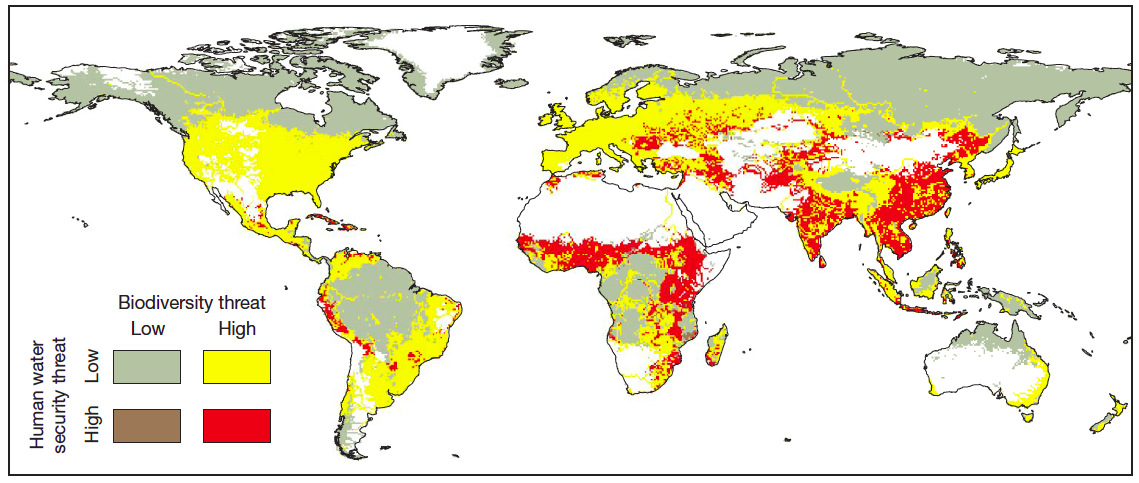
\includegraphics[width=1\textwidth]{images/waterthreat.png}\\
  \raggedright \footnotesize Vörösmarty et al., 2010. Nature \normalsize
  \pause
  \vspace{3pt}
  \begin{itemize}
  \item 55\% decline in 300 freshwater species \footnotesize (UNEP, 2015; WWF, 2015)
  \normalsize
  \pause
  \item significant decrease of discharge\\
  in 23\% world’s largest streams \footnotesize (Dai et al., 2009. J. Clim.)
  \end{itemize}
\end{frame}

%%%%%%%%%%%%%%%%%%%%%%%%%%% Slide 2 %%%%%%%%%%%%%%%%%%%%%%%%%

\begin{frame}[fragile]
  \frametitle{Freshwater degradation is triggered \protect\\ by four groups of stressors}
  \centering
    \only<1> {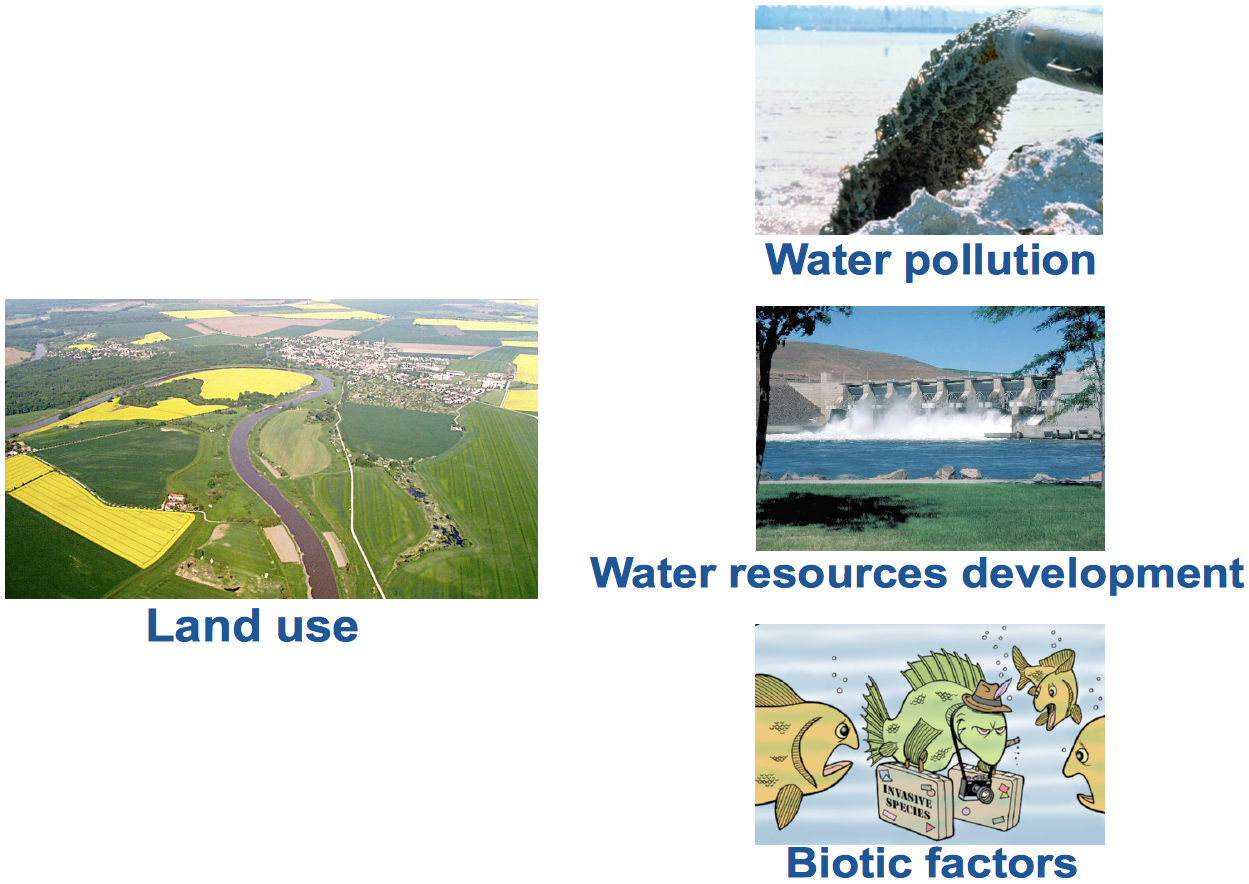
\includegraphics[width=0.85\textwidth]{images/Stressors.png}\\
     \hspace{3cm} \footnotesize Vörösmarty et al., 2010. Nature; Dudgeon et al., 2005. Bio. Rev.}
     \only<2> {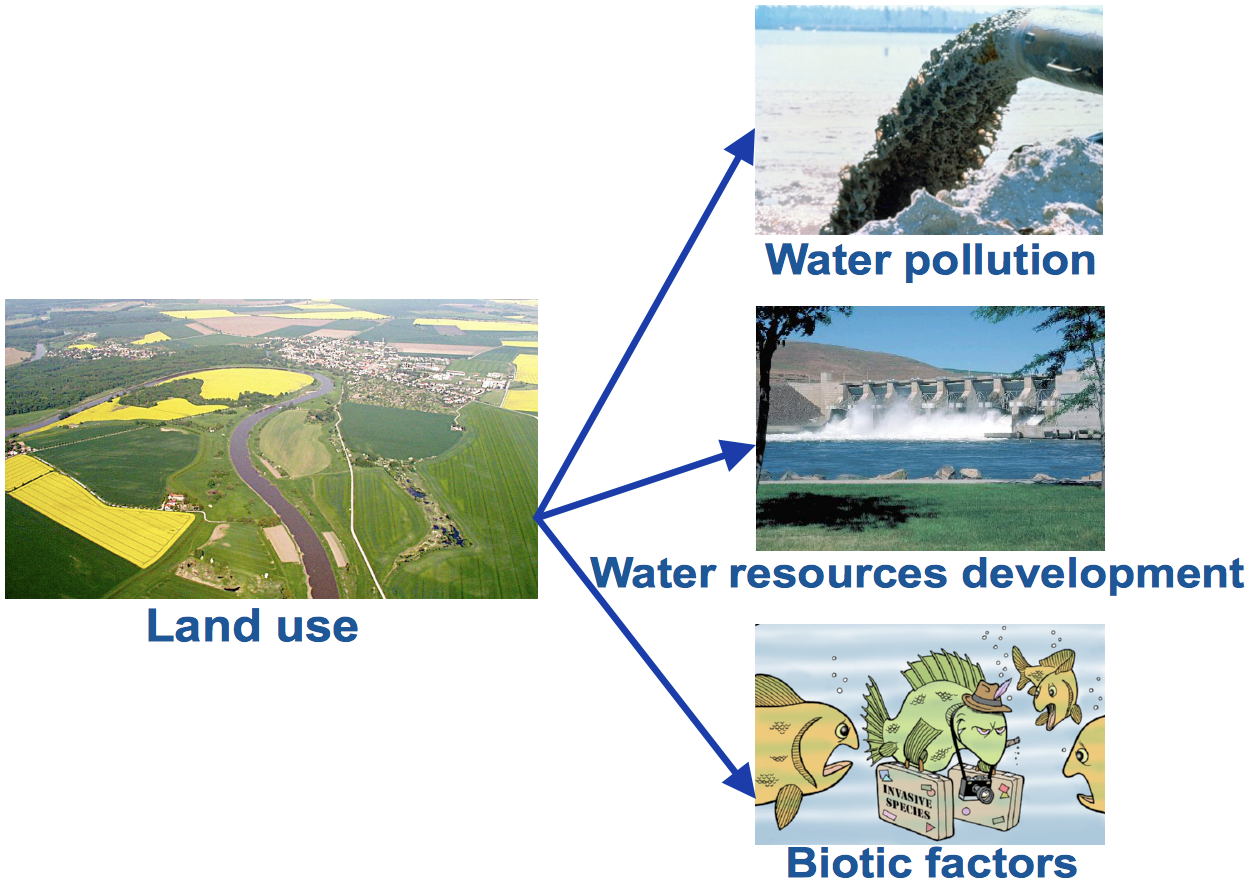
\includegraphics[width=0.85\textwidth]{images/SLink.png}\\
     \hspace{3cm} \footnotesize Vörösmarty et al., 2010. Nature; Dudgeon et al., 2005. Bio. Rev.}
    \only<3> {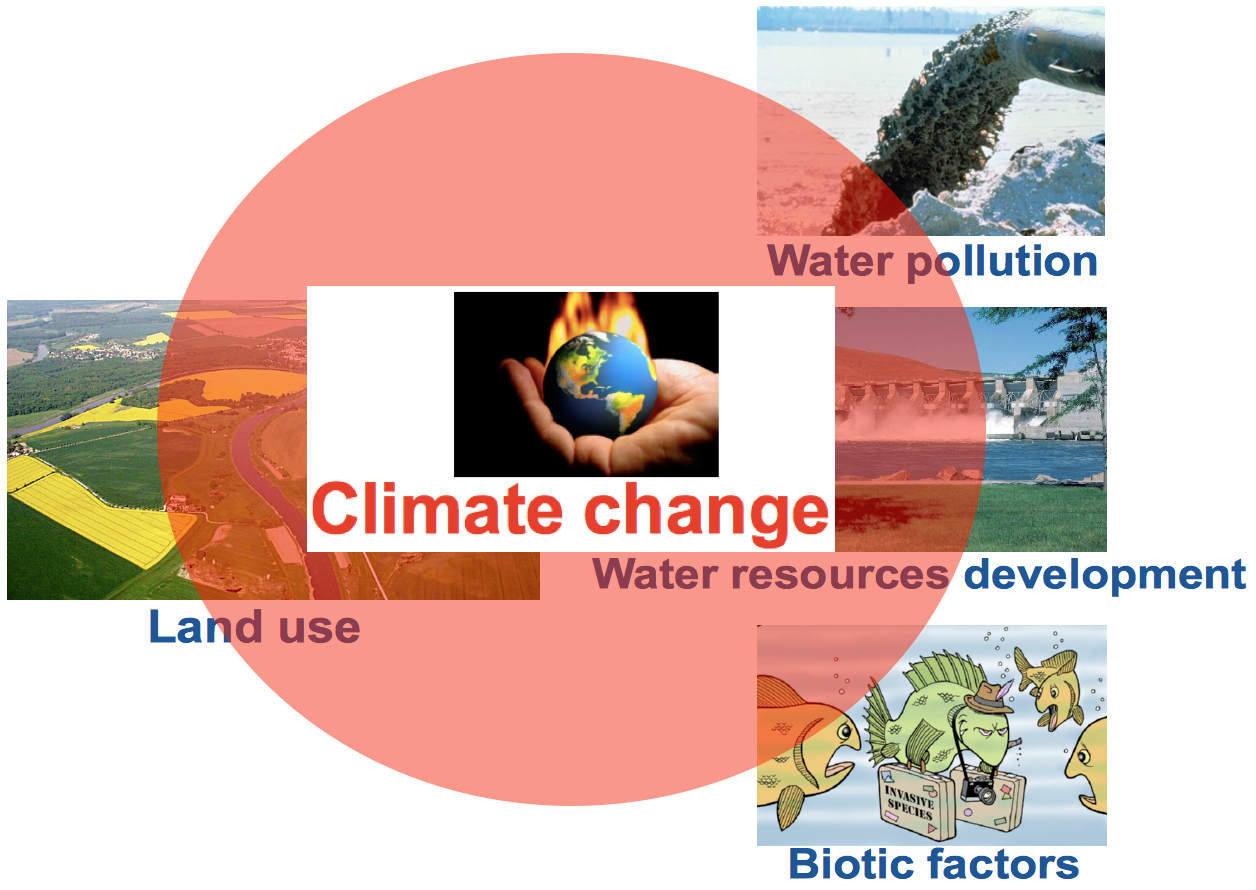
\includegraphics[width=0.85\textwidth]{images/SClimate.png}\\
    \hspace{3cm} \footnotesize Vörösmarty et al., 2010. Nature; Dudgeon et al., 2005. Bio. Rev.}
\end{frame}


%%%%%%%%%%%%%%%%%%%%%%%%%%% Slide 3 %%%%%%%%%%%%%%%%%%%%%%%%%

%\begin{frame}[fragile]
  %\frametitle{Risks of exceeding Planetary boundaries \protect\\ for Land use and Climate Change}
  %\centering
    %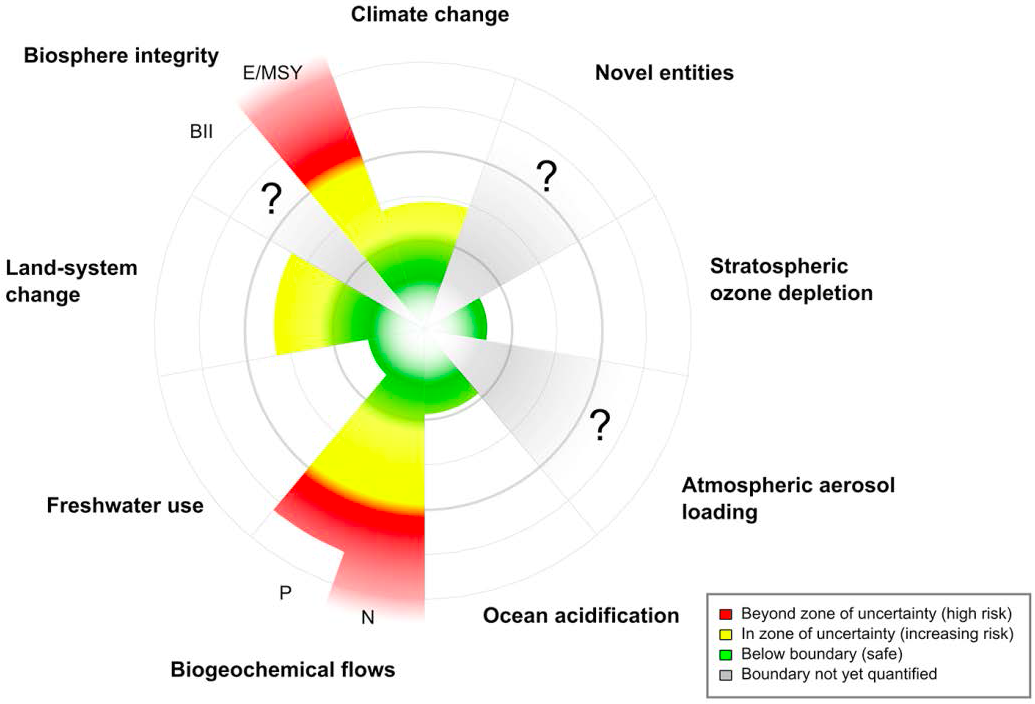
\includegraphics[width=0.9\textwidth]{images/PB.png}\\
      %\hspace{7cm} \footnotesize Steffen et al., 2015. Science
%\end{frame}

%%%%%%%%%%%%%%%%%%%%%%%%%%% Slide 4 %%%%%%%%%%%%%%%%%%%%%%%%%

%\begin{frame}[fragile]
  %\frametitle{Unprecedented impacts on humans and ecosystems}
  %\begin{itemize}
  %\item \alert{upto 37\%} loss of freshwater biodiversity
  %\smallskip
  %\pause
  %\item \alert{2/3 of world’s population}, especially inhabitants of developing countries, in moderate to severe water stress
  %\end{itemize}\\
  %\hspace{3.5cm} \footnotesize UNEP, 2015; WWF, 2015; Vörösmarty et al., 2010. Nature \LARGE \\ \\ \\
  %\alert{Response?}
%\end{frame}

%%%%%%%%%%%%%%%%%%%%%%%%%%% Slide 5 %%%%%%%%%%%%%%%%%%%%%%%%%

\begin{frame}[fragile]
  \frametitle{Response:\protect\\Political frameworks aims at preservation and restoration}
  \begin{columns}
  \column{5cm}
  \onslide<1-> \centering \textbf{Developed countries}\\
  \vspace{10pt}
  \onslide<2-> {
\includegraphics[width=0.7\textwidth]{images/WFD.png}\\
     \hspace{2cm} \footnotesize EC, 2010\\ \normalsize
     \medskip
     \raggedright \alert{Local scale approaches}}
  \column{5cm}
  \onslide<1-> \centering \textbf{Developing countries}\\
  \vspace{16pt}
  \onslide<3-> {\Large{\alert{No such framework!}} \\
     \hspace{1cm} \footnotesize MEPA China, 2014; UNEP, 2008\\ \normalsize
     \vspace{20pt}
     \raggedright \alert{Data scarcity}}
  \end{columns}\\
  \vspace{15pt}
  \onslide<4> \hspace{2cm} \LARGE \alert{Large Scale approaches}
\end{frame}

%%%%%%%%%%%%%%%%%%%%%%%%%%% Slide 6 %%%%%%%%%%%%%%%%%%%%%%%%%

\begin{frame}[fragile]
  \frametitle{Large scale approaches can complement \protect\\ small scale approaches}
  \begin{itemize}
  \item Local and regional species richness often exhibit positive relationships \footnotesize (Heino et al., 2013. Fresh. Bio.; Hugueny et al., 2010. Am. Fish. Soc. Symp.) \normalsize
  \smallskip
  \pause
  \item Integrated and transboundary freshwater management \footnotesize (EC, 2010) \normalsize
  \smallskip
  \pause
  \item Data-gap filling by novel methods and available secondary datasets \footnotesize (Hengl, 2009. Geostat. Map.; Törnqvist et al., 2011. Env.Int.) \normalsize
  \end{itemize}
\end{frame}

%%%%%%%%%%%%%%%%%%%%%%%%%%% Slide 7 %%%%%%%%%%%%%%%%%%%%%%%%%

\begin{frame}[fragile]
  \frametitle{Spatial Models are indispensable tools \protect\\ for large scale ecological analyses}
  \begin{columns}
  \column{5cm}
  \onslide<1-> {\vspace{-1.2cm}\\\centering \textbf{Geographic Information Systems (GIS)}\\}
  \vspace{5pt}
  \onslide<2-> {\alert{Spatial attributes (x,y), z} \\
     \hspace{1cm} \footnotesize Fortin and Dale, 2005. Sp. Anal.\\ \normalsize
     \vspace{5pt}
     \raggedright \begin{itemize}
     \item Answers to Location and Scale related questions\\
     \item Integration and processing of large datasets\\
     \end{itemize}\\ \vspace{10pt}}
     \onslide<6> {\alert{\Large Integration with Ecological Models}}
  \column{5cm}
  \onslide<3-> {\vspace{2pt}\\ \centering \textbf{Spatial Statistics}\\}
  \vspace{5pt}
  \onslide<4-> {\alert{Statistics for spatial data}\\
     \hspace{1cm} \footnotesize Legendre, 1993. Ecol.\\ \normalsize
     \vspace{5pt}}
     \onslide<5->{\raggedright \begin{itemize}
     \item Spatial autocorrelation
     \end{itemize}\\
     \vspace{5pt}
     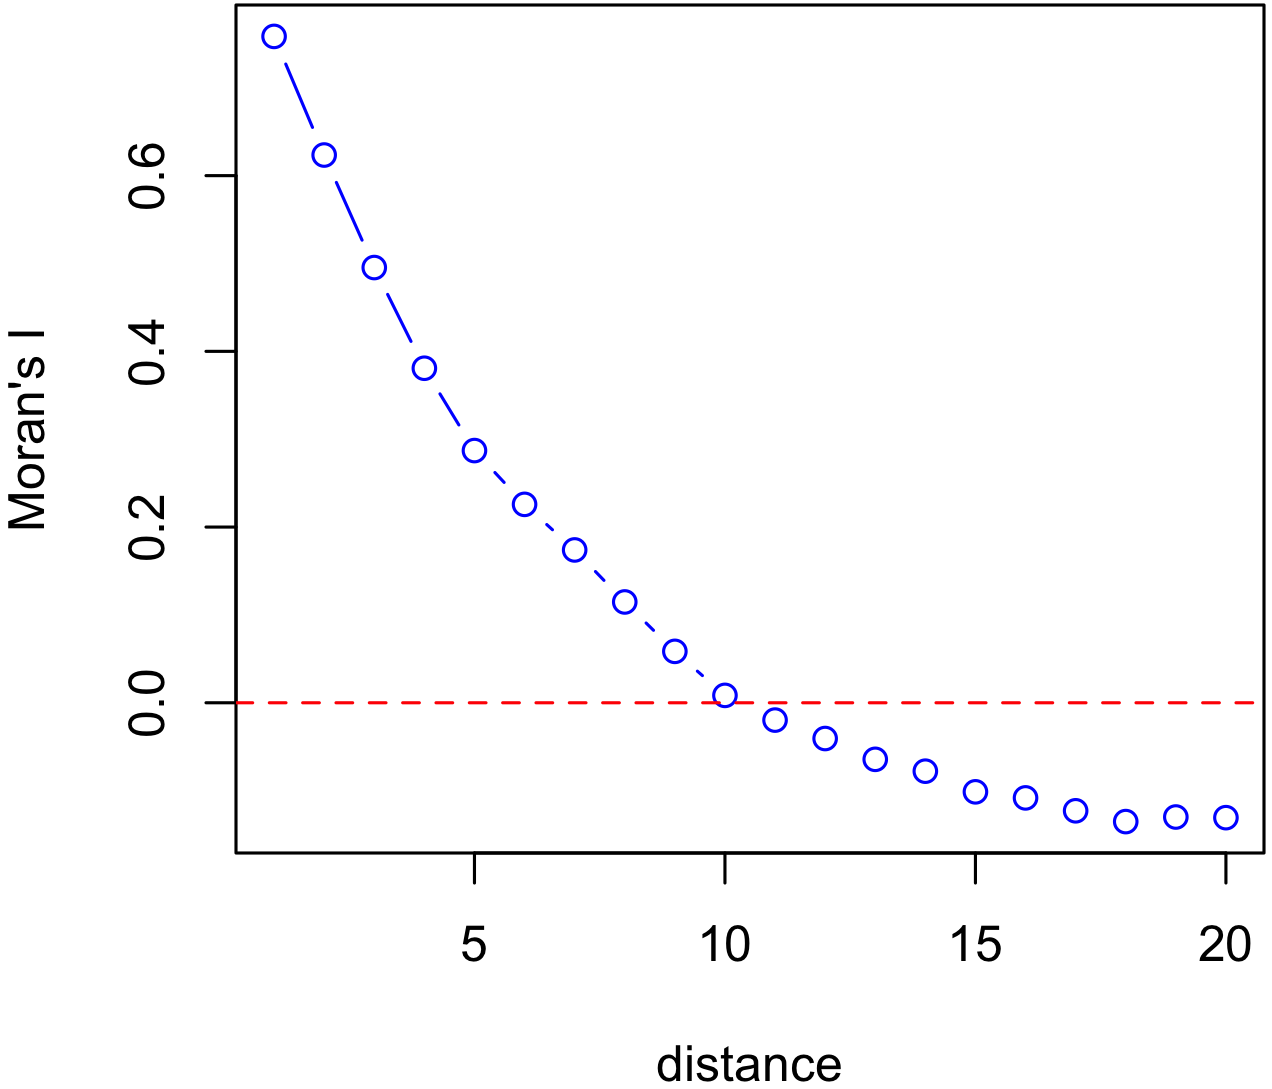
\includegraphics[width=1.05\textwidth]{images/spcorr.png}
     }
  \end{columns}
\end{frame}

%%%%%%%%%%%%%%%%%%%%%%%%%%% Slide 8 %%%%%%%%%%%%%%%%%%%%%%%%%

\begin{frame}
  \frametitle{My Ph.D. thesis envelops four studies \protect\\ developing and integrating spatial and ecological models}
  \centering
  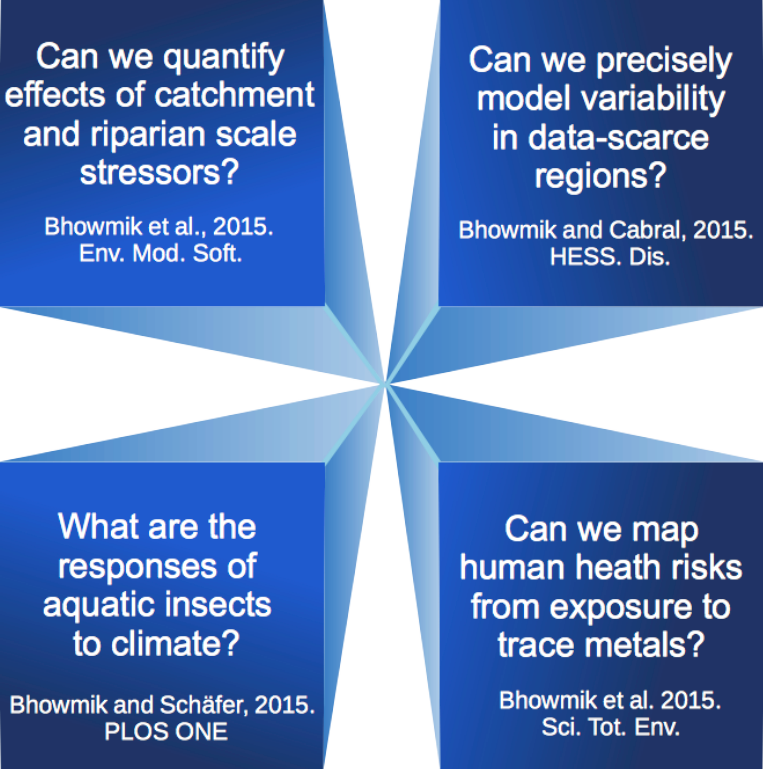
\includegraphics[width=0.68\textwidth]{images/Studies.png}
  %\begin{columns}
  %\column{5cm}
  %\\\vspace{2pt}
  %\centering
  %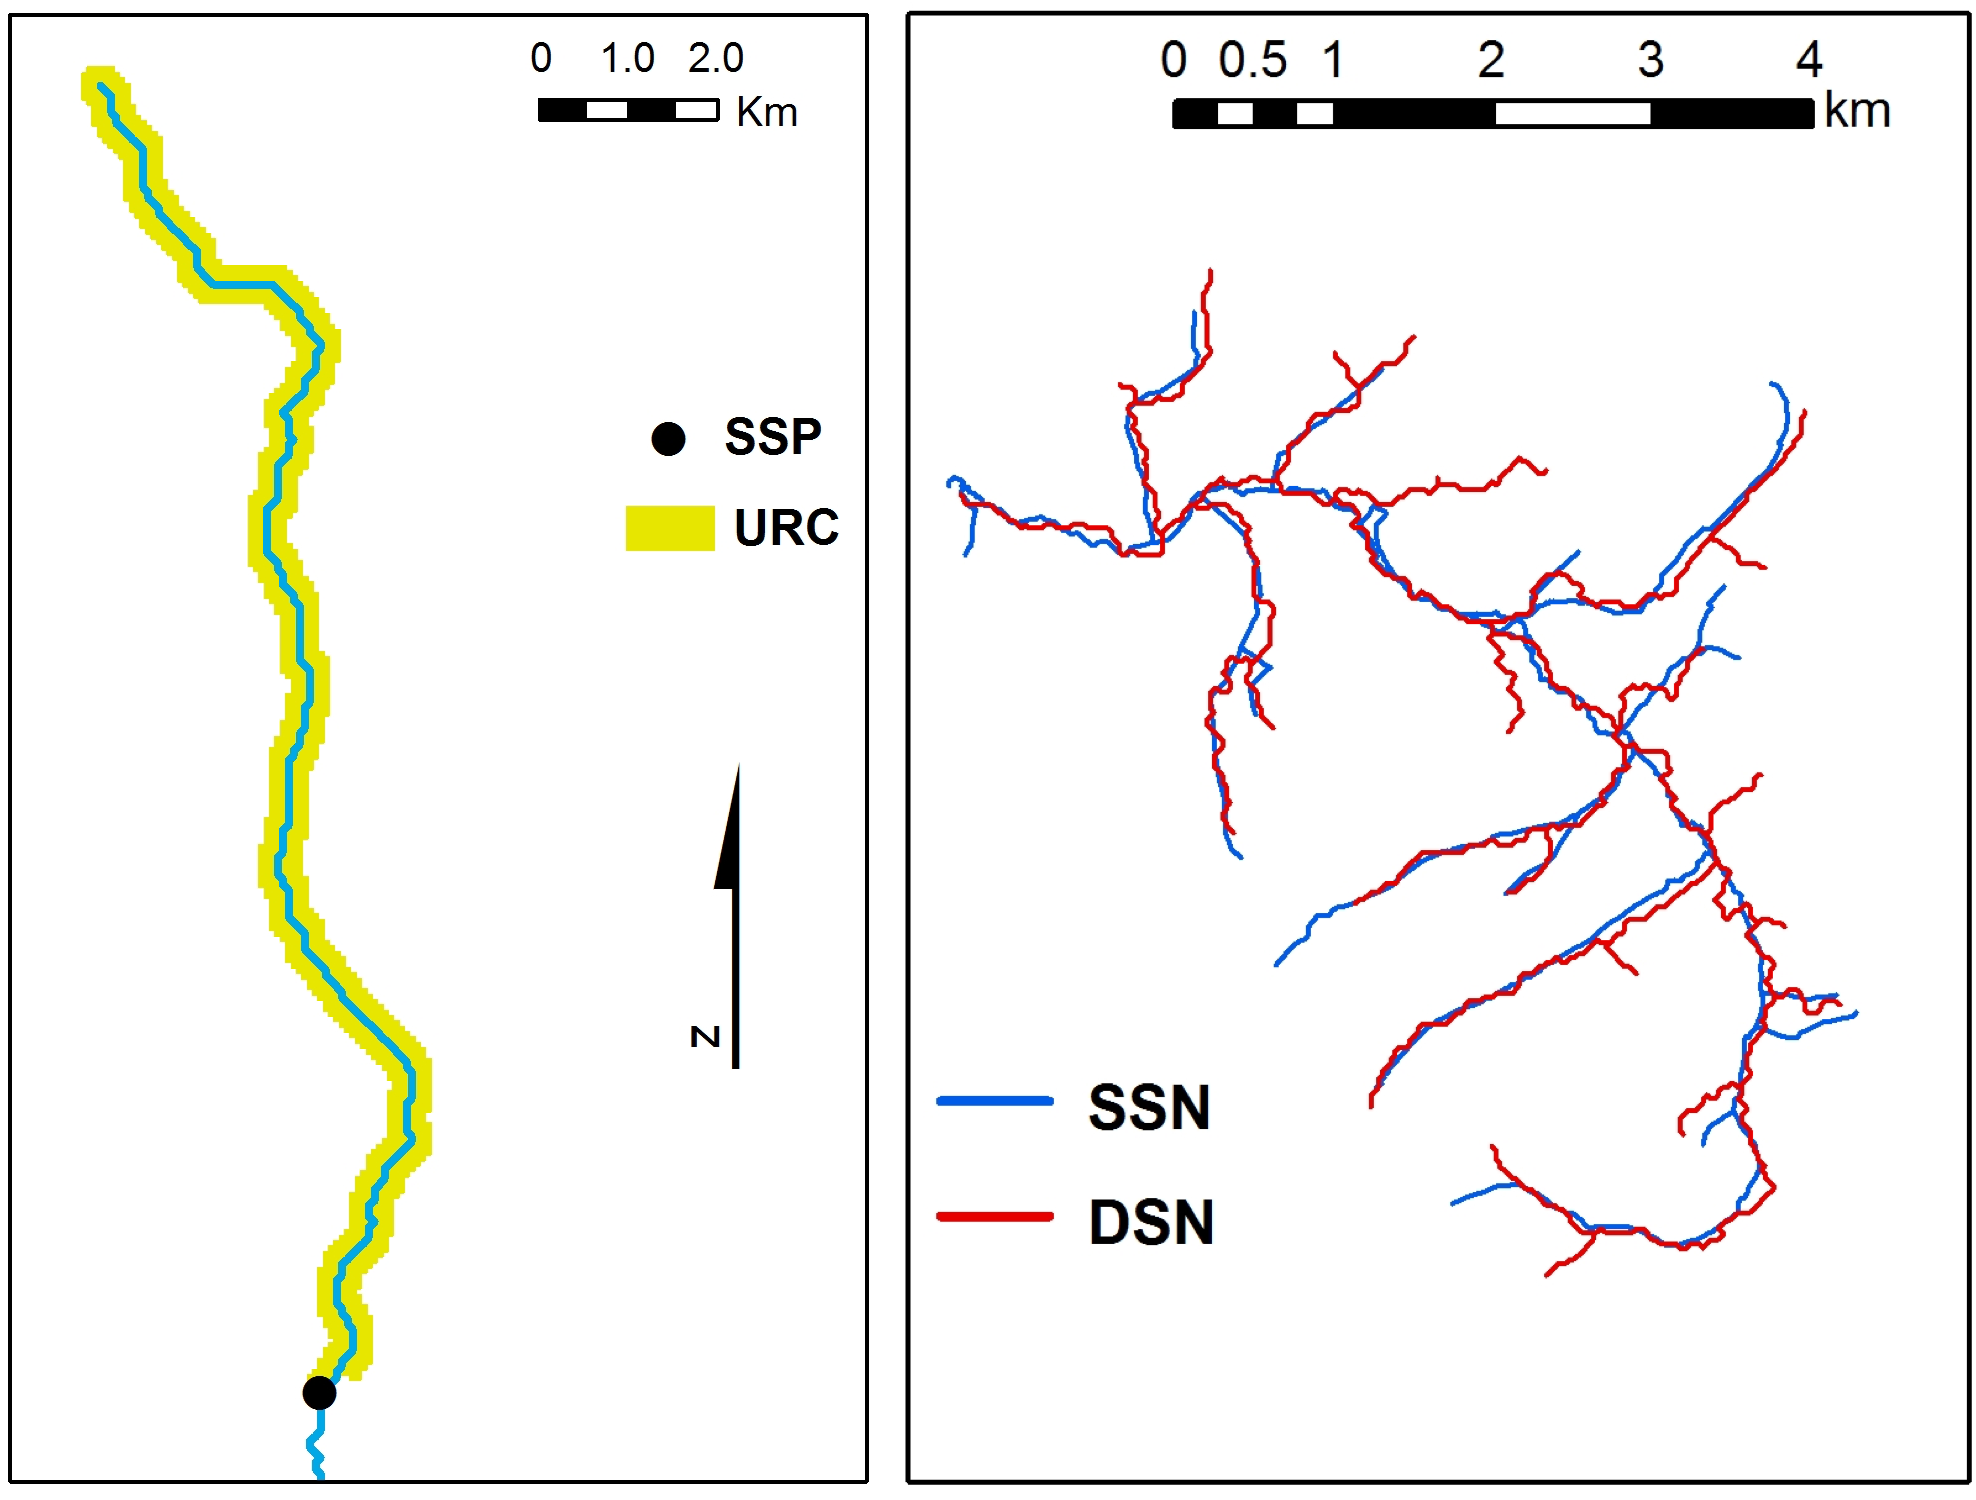
\includegraphics[width=0.8\textwidth]{images/St1.png}\\
  %\footnotesize Bhowmik et al., 2015. Env. Mod. Soft.\\
  %\vspace{2pt}
  %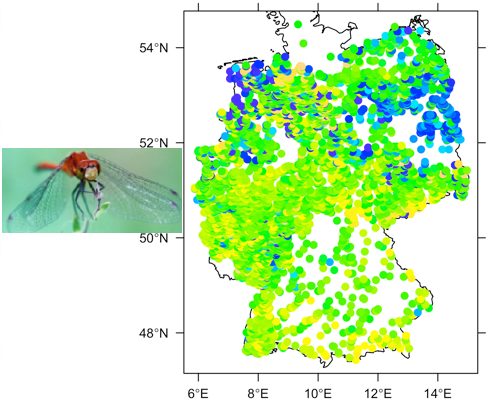
\includegraphics[width=0.6\textwidth]{images/St3.png}\\
   % \footnotesize Bhowmik and Schäfer, 2015. PLOS ONE
  %\column{5cm}
  %\\\vspace{2pt}
  %\centering
  %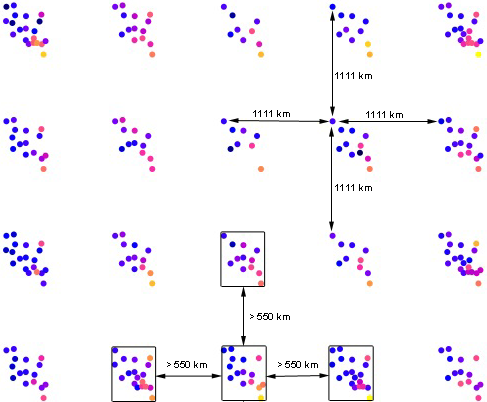
\includegraphics[width=0.8\textwidth]{images/St2.png}\\
  %\vspace{4pt}
  %\footnotesize Bhowmik and Cabral, 2015. HESS. Dis.\\
  %\vspace{4pt}
  %\includegraphics[width=0.88\textwidth]{images/St4.png}\\
  %\footnotesize Bhowmik and Schäfer, 2015. PLOS ONE
  %\end{columns}
\end{frame}

%%%%%%%%%%%%%%%%%%%%%%%%%%%%%%%%%%%%%%%%%%%%%%%%%%%%%%%%%%%%%

%%%%%%%%%%%%%%%%%%%%%%%%%%% Slide 9 %%%%%%%%%%%%%%%%%%%%%%%%%

\plain{}{\Large Quantifying catchment and riparian scale stressors\\ \vspace{0.5cm}
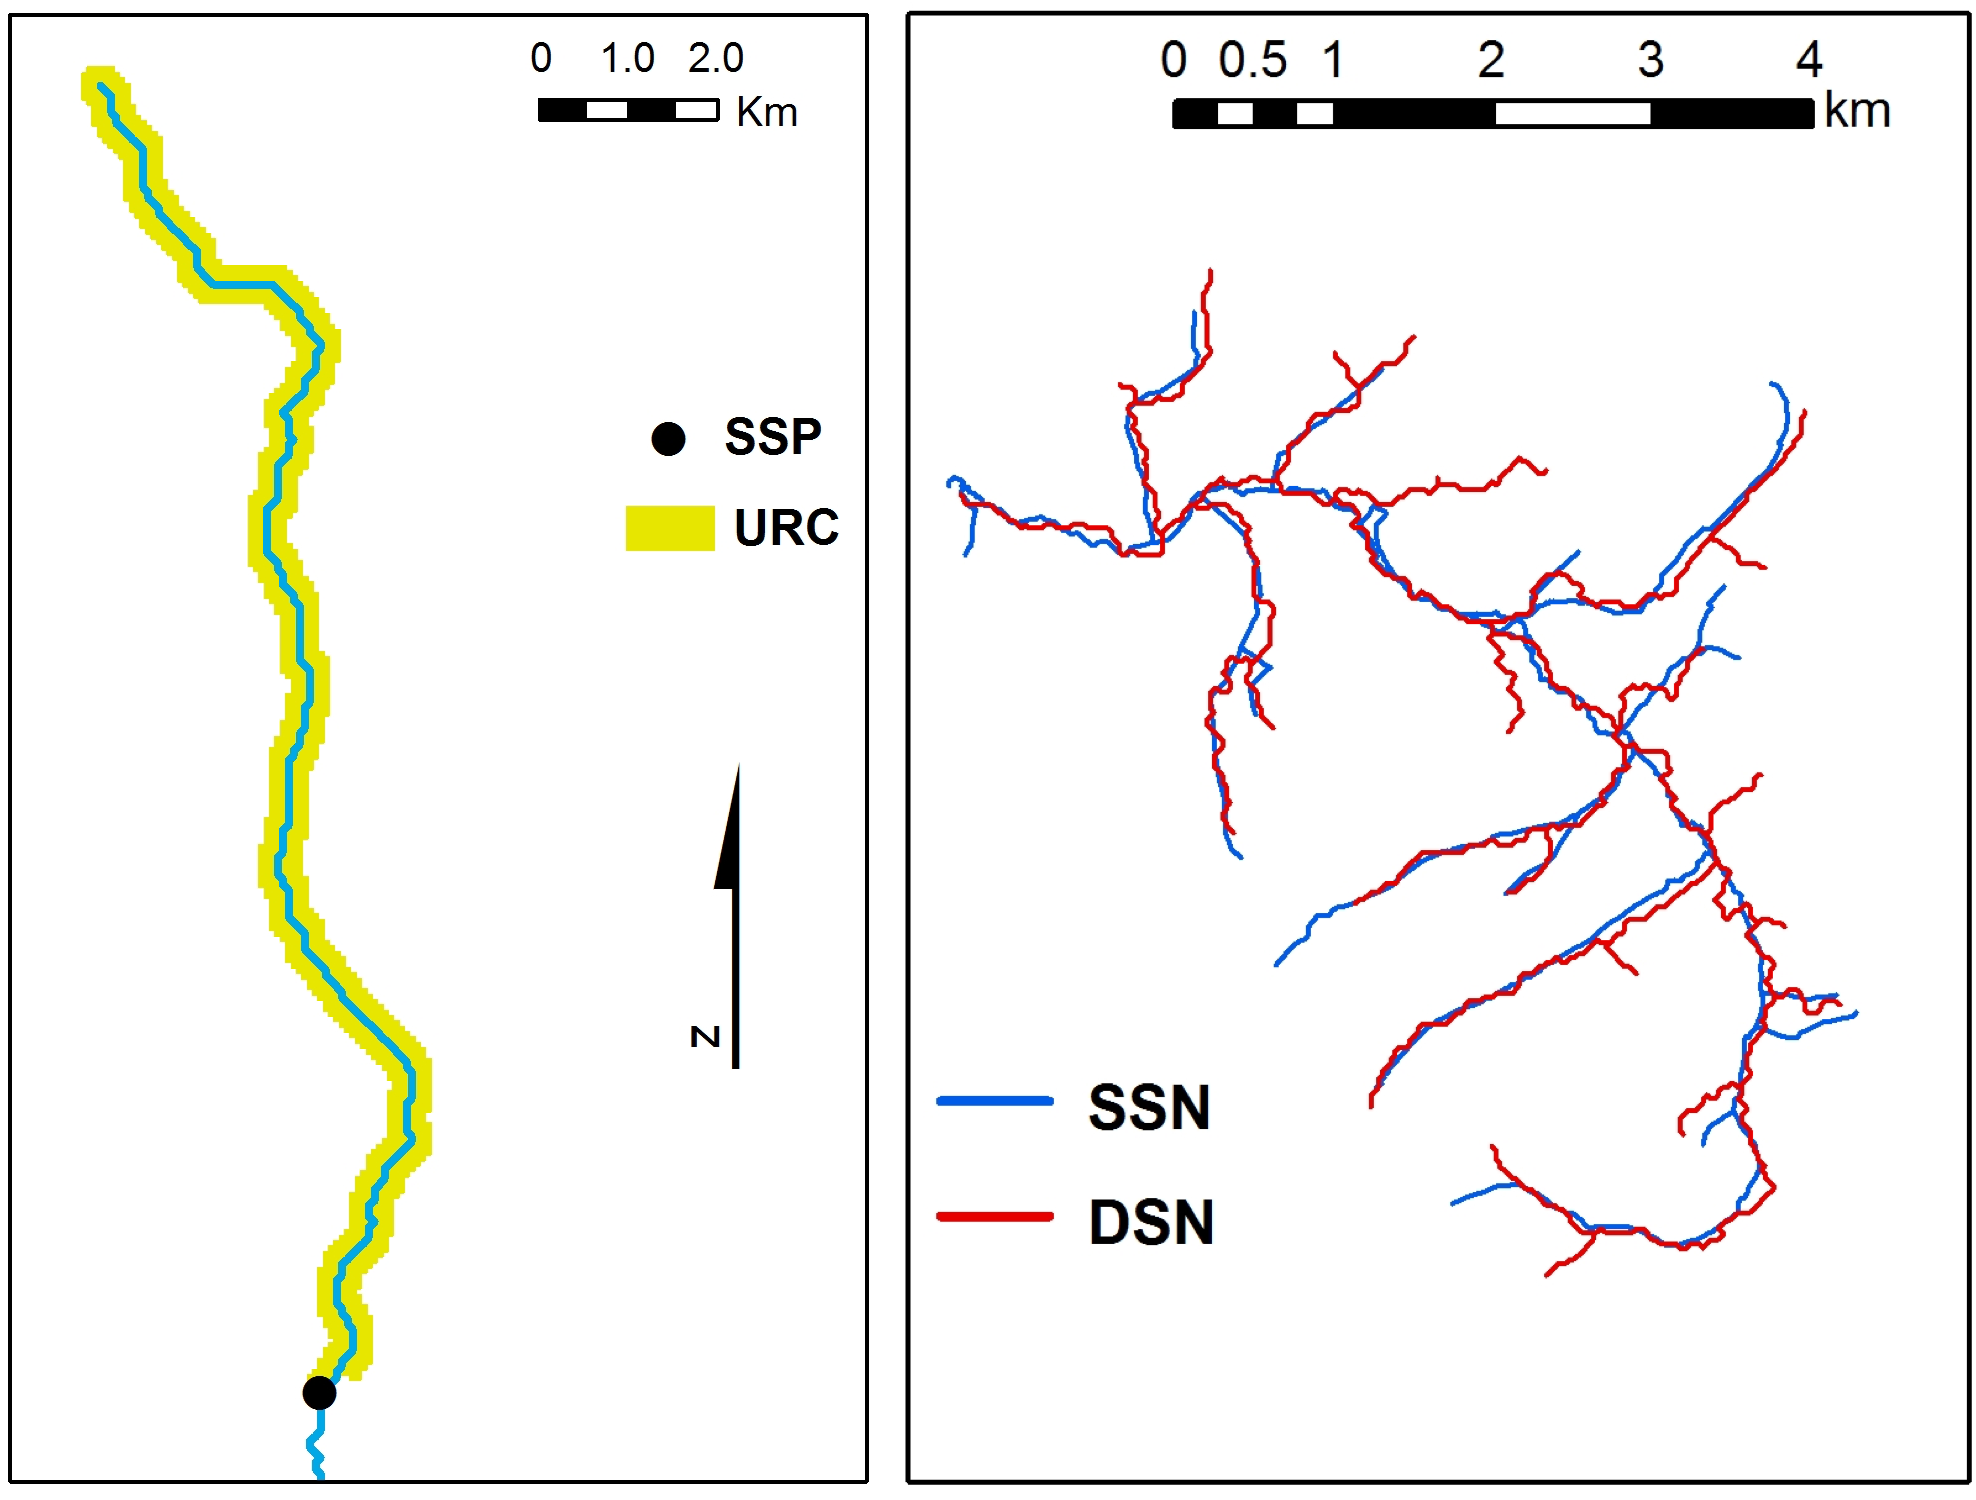
\includegraphics[width=0.6\textwidth]{images/St1.png}\\
\normalsize Bhowmik et al., 2015. Env. Mod. Soft., 63: 240-250}

%%%%%%%%%%%%%%%%%%%%%%%%%%% Slide 10 %%%%%%%%%%%%%%%%%%%%%%%%%

\begin{frame}
  \frametitle{Automated Accumulation Threshold selection \protect\\ and RIparian Corridor delineation (ATRIC)}
  \centering \vspace{4pt}
    \only<1> {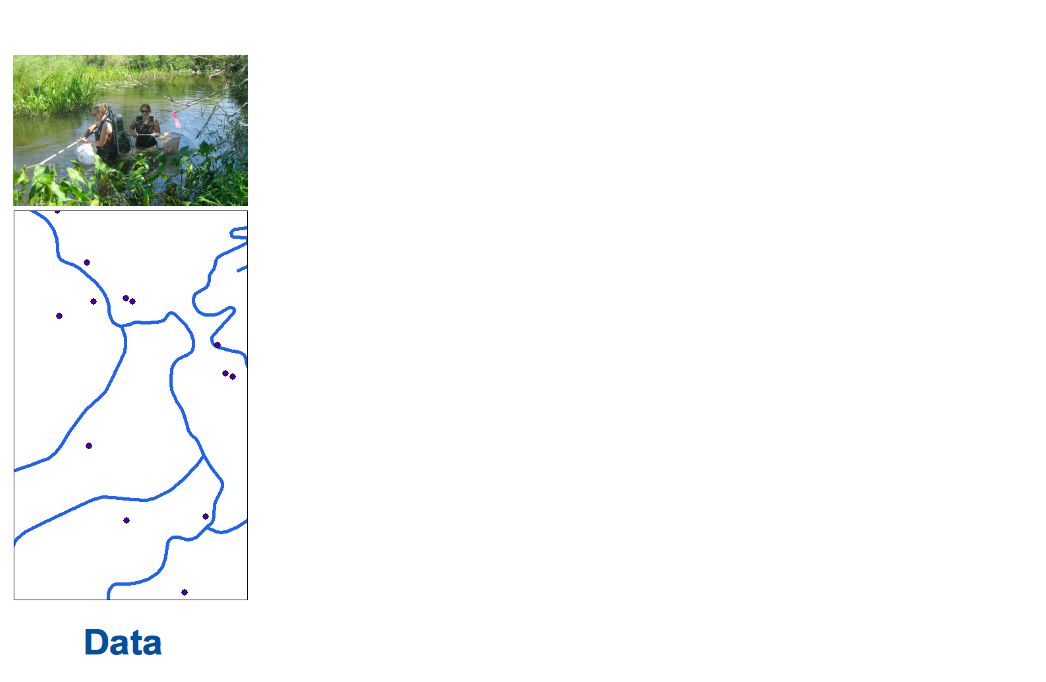
\includegraphics[width=1.05\textwidth]{images/ATRIC1.png}}\\
    \only<2> {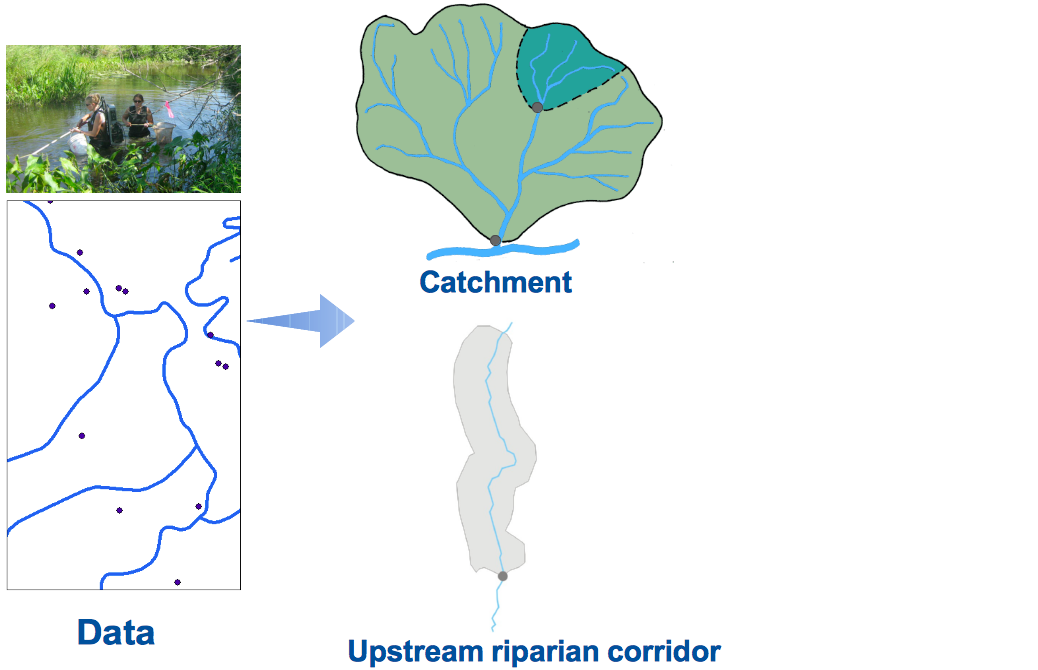
\includegraphics[width=1.05\textwidth]{images/ATRIC2.png}}\\
    \only<3> {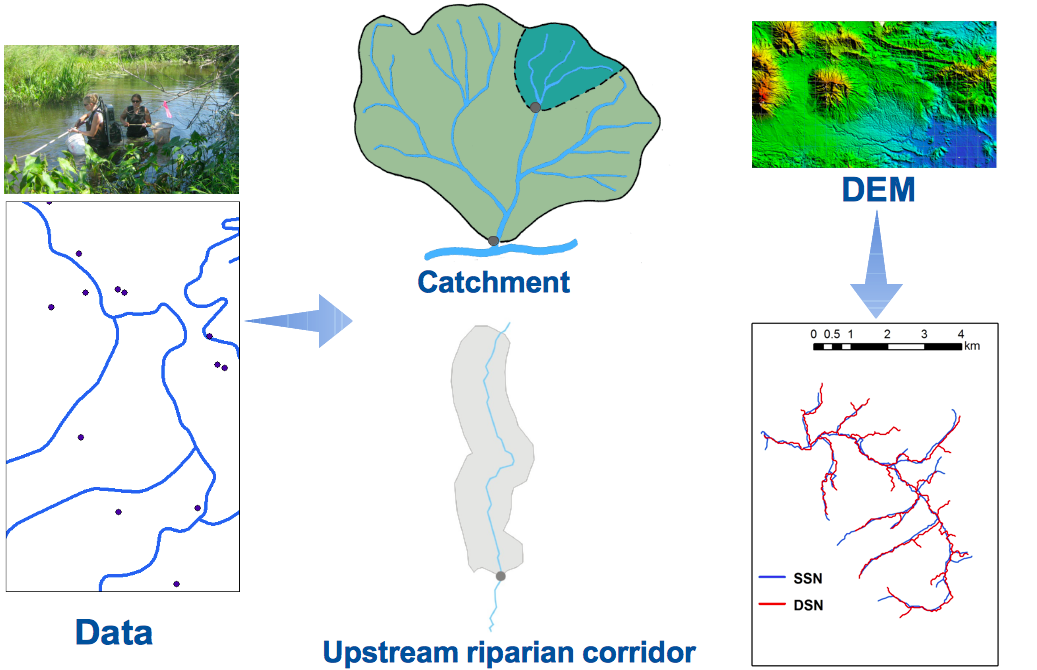
\includegraphics[width=1.05\textwidth]{images/ATRIC3.png}}\\
\end{frame}

%%%%%%%%%%%%%%%%%%%%%%%%%%% Slide 10 %%%%%%%%%%%%%%%%%%%%%%%%%

\begin{frame}
  \frametitle{Automated Accumulation Threshold selection \protect\\ and RIparian Corridor delineation (ATRIC)}
  \centering
    \onslide<1-> {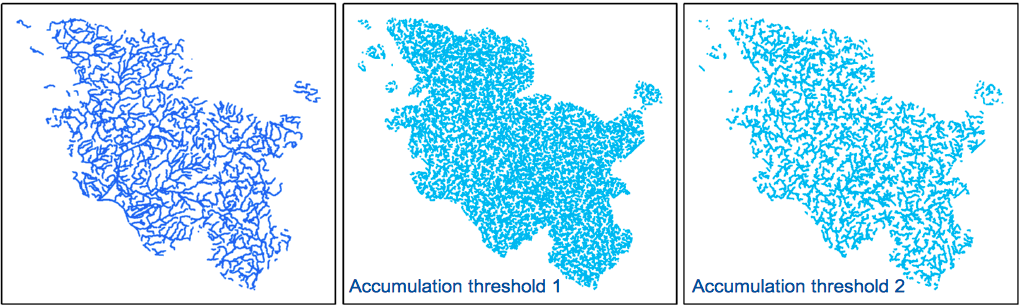
\includegraphics[width=0.85\textwidth]{images/AT.png}}\\
    \onslide<2->{\alert{Trial and error!} \footnotesize (Tarboton et al., 1991. Hydrol. Process.)\normalsize}\\
    \onslide<3-> {
\includegraphics[width=0.35\textwidth]{images/TE.png}\hspace{1cm}\alert{subjective}\hspace{1cm}\alert{laborious}}\\\vspace{2pt}
    \onslide<4>{\raggedright - Available algorithms: \alert{(i) for small scale data (ii) inaccessible}\\
    \hspace{1cm} \footnotesize (Lin et al., 2006. Hydrol. Process.; Heine et al., 2004. Ann. Assoc. Am. Geogr.)}
\end{frame}

%%%%%%%%%%%%%%%%%%%%%%%%%%%%%%%%%%%%%%%%%%%%%%%%%%%%%%%%%%%%%

%%%%%%%%%%%%%%%%%%%%%%%%%%% Slide 11 %%%%%%%%%%%%%%%%%%%%%%%%%

\plain{}{\Large Modelling spatial variability with precision\\ \vspace{0.5cm}
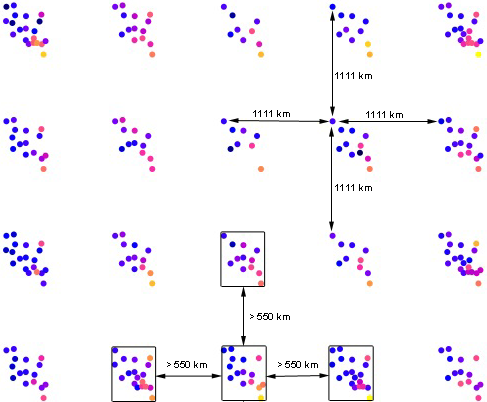
\includegraphics[width=0.6\textwidth]{images/St2.png}\\
\normalsize Bhowmik and Cabral, 2015. HydroESS. Dis., 12: 2243-2265}

%%%%%%%%%%%%%%%%%%%%%%%%%%% Slide 12 %%%%%%%%%%%%%%%%%%%%%%%%%

\begin{frame}
  \frametitle{Spatially Shifting Temporal Points (SSTP)}
  \only<1>
  {\begin{columns}
  \column{5cm}
    \centering
    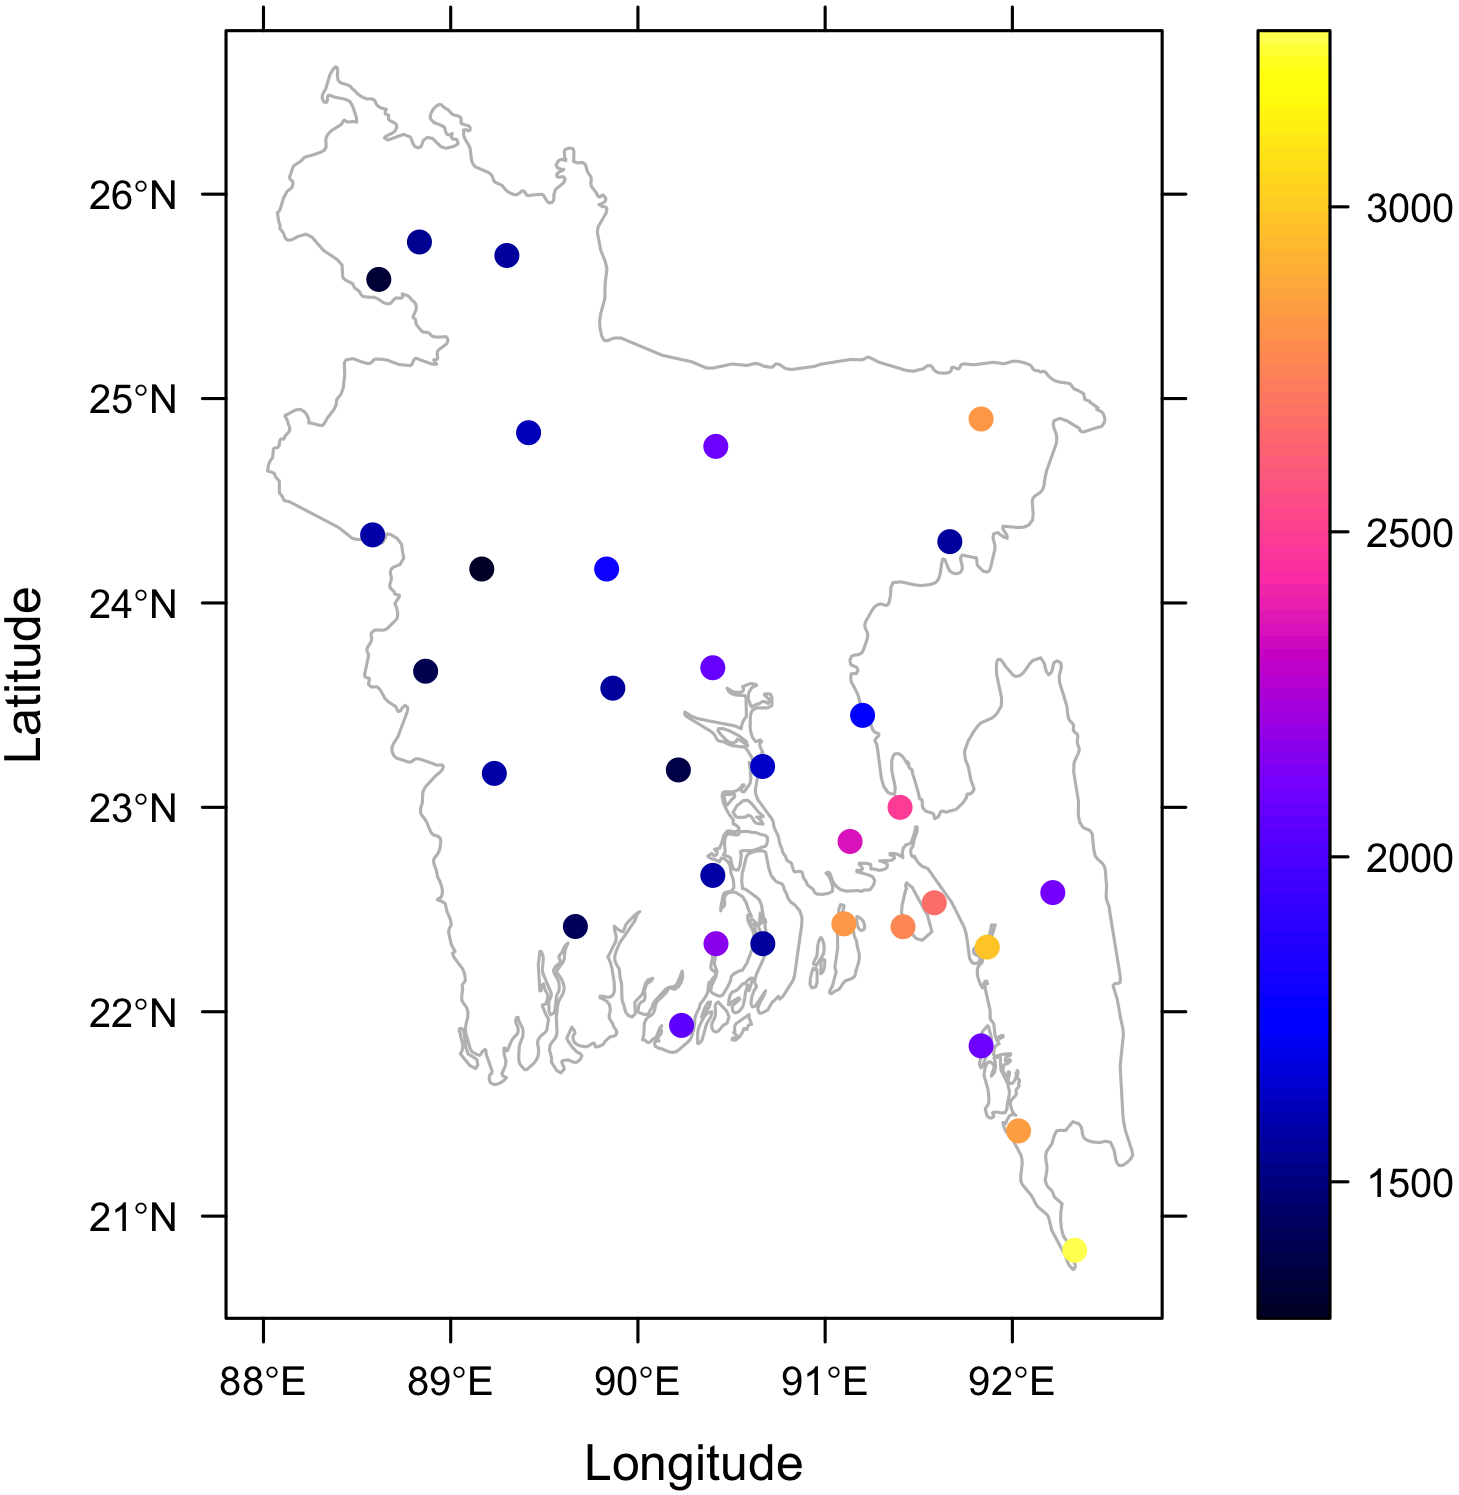
\includegraphics[width=1.15\textwidth]{images/SSTP6.png}
    \column{5cm}
    \centering
    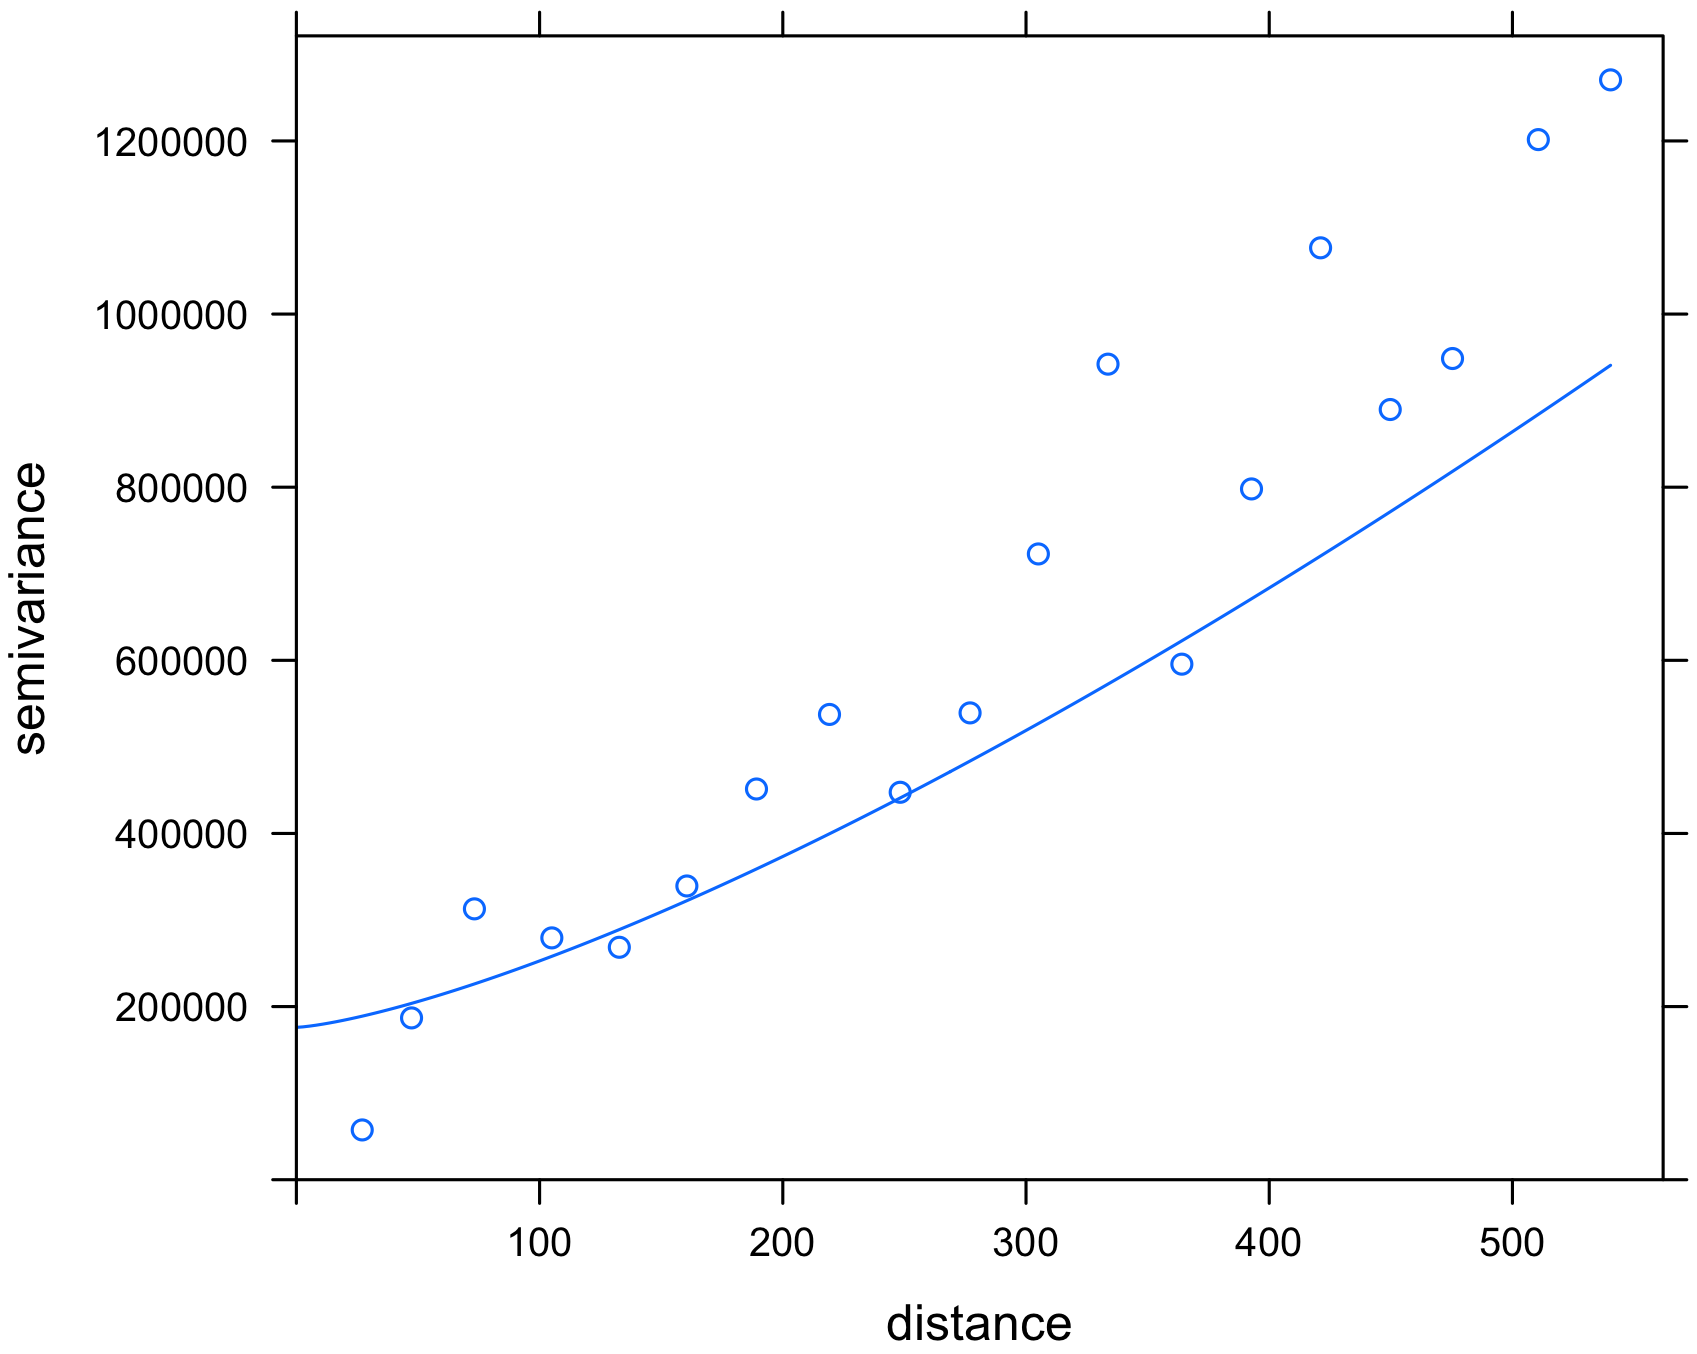
\includegraphics[width=1.15\textwidth]{images/SSTP1.png}
    \end{columns}\\
  \hspace{5cm} \footnotesize Webster and Oliver, 2007. Geostat. Env. Sci.}
  \only<2>
  {\begin{columns}
  \column{5cm}
    \centering
    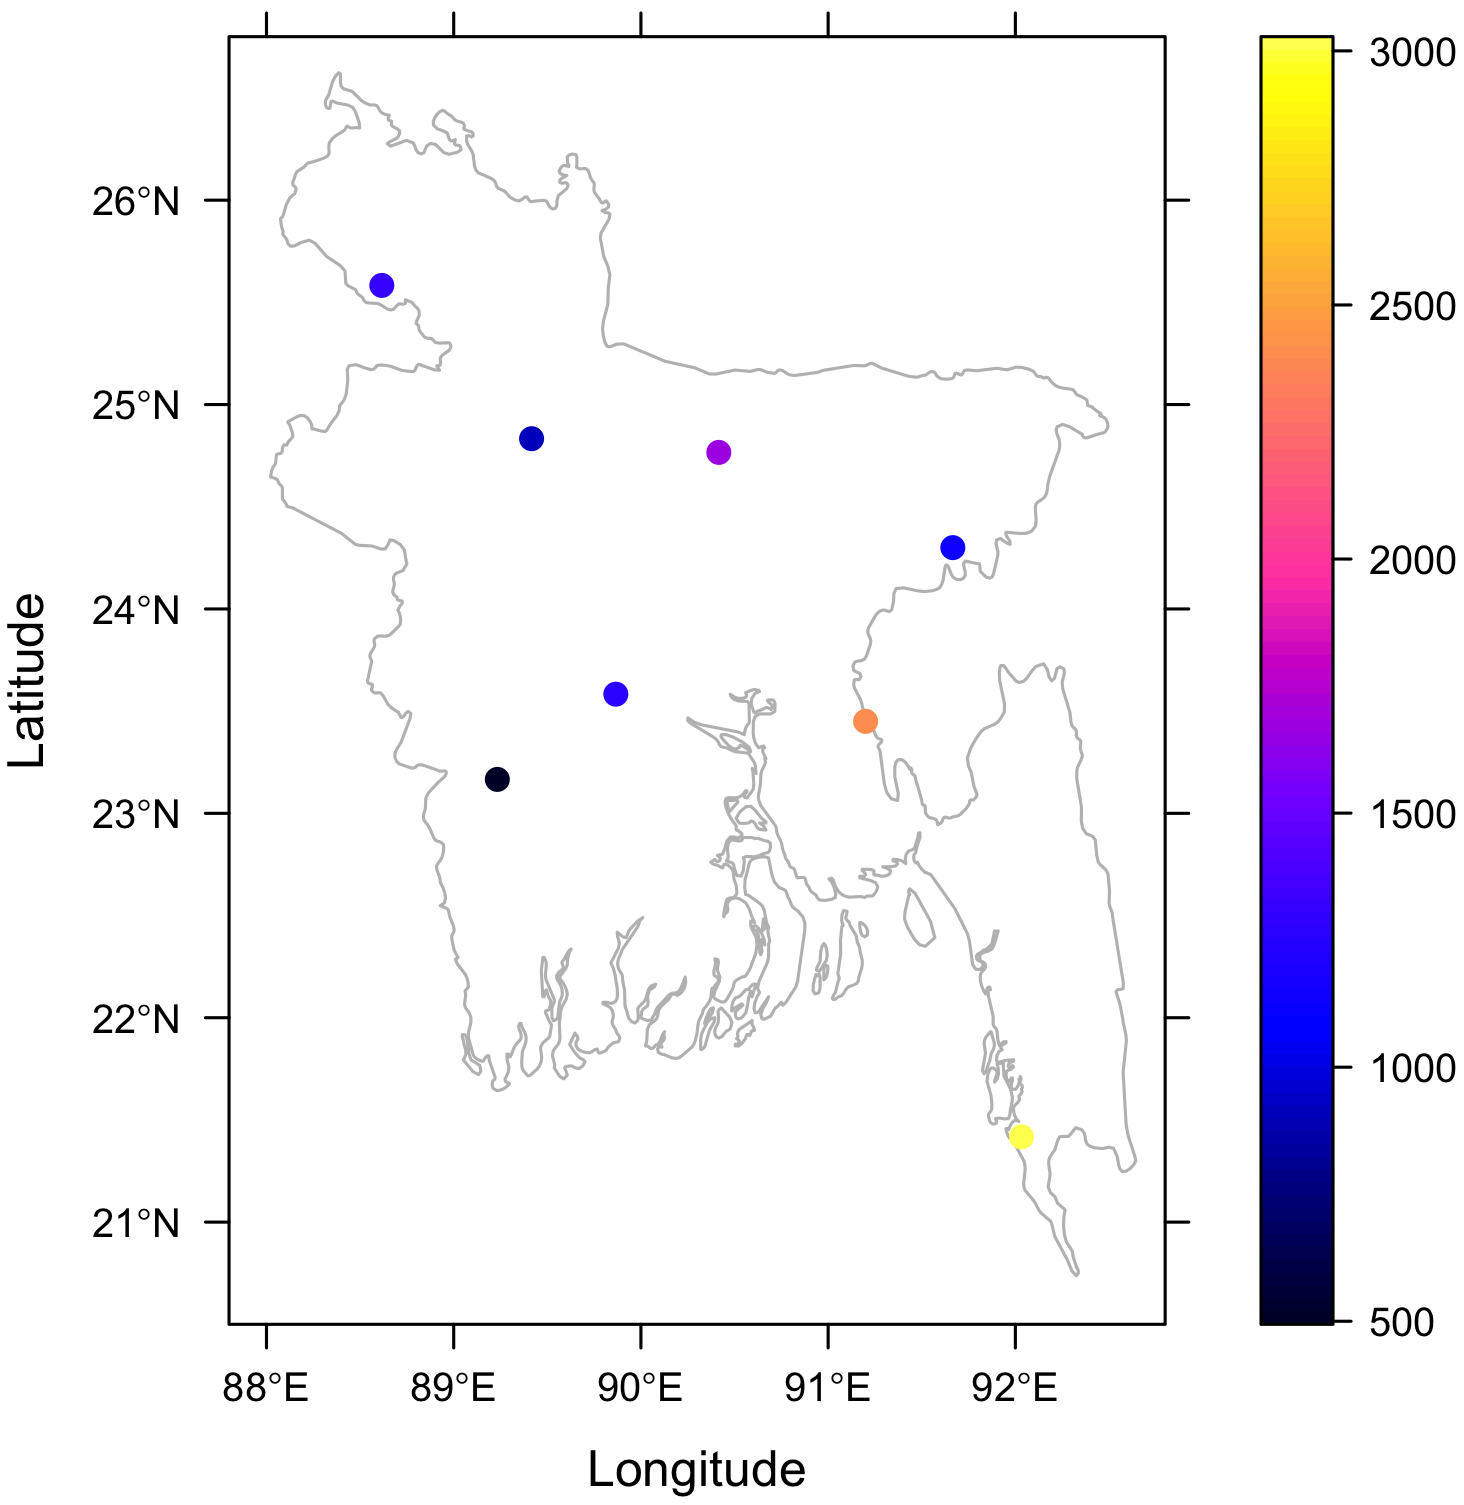
\includegraphics[width=1.15\textwidth]{images/SSTP2.png}
    \column{5cm}
    \centering
    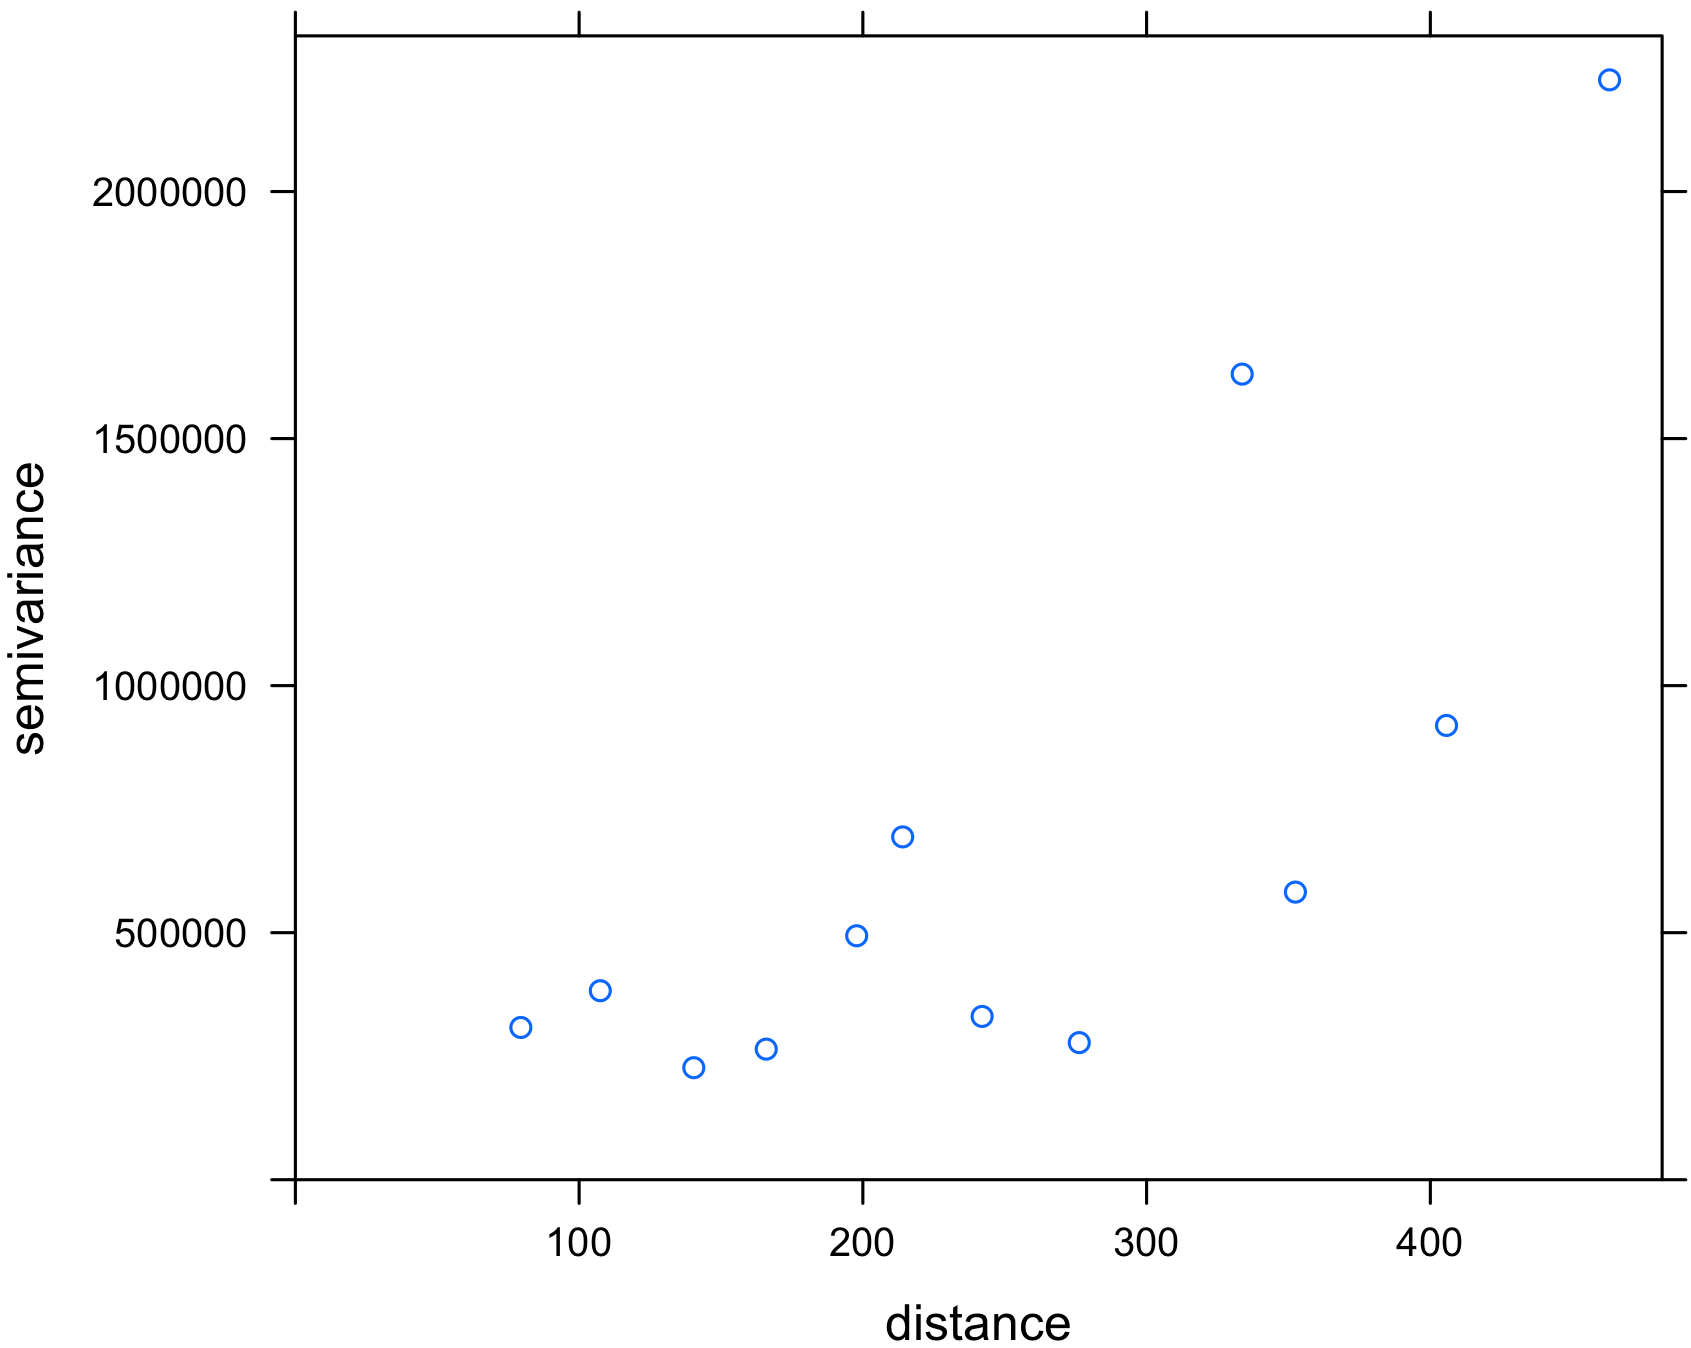
\includegraphics[width=1.15\textwidth]{images/SSTP3.png}
    \end{columns}\\
  \hspace{3cm} \footnotesize Oliver, 2010. Var. Krig.; Truong et al., 2012. Comp. Geosci.}
    \only<3>
  {\begin{columns}
  \column{5cm}
    \centering
    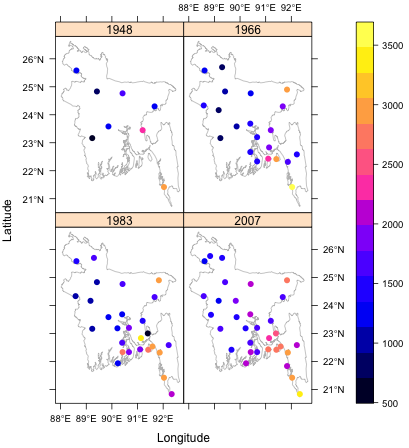
\includegraphics[width=1.15\textwidth]{images/SSTP4.png}
    \column{5cm}
    \centering
    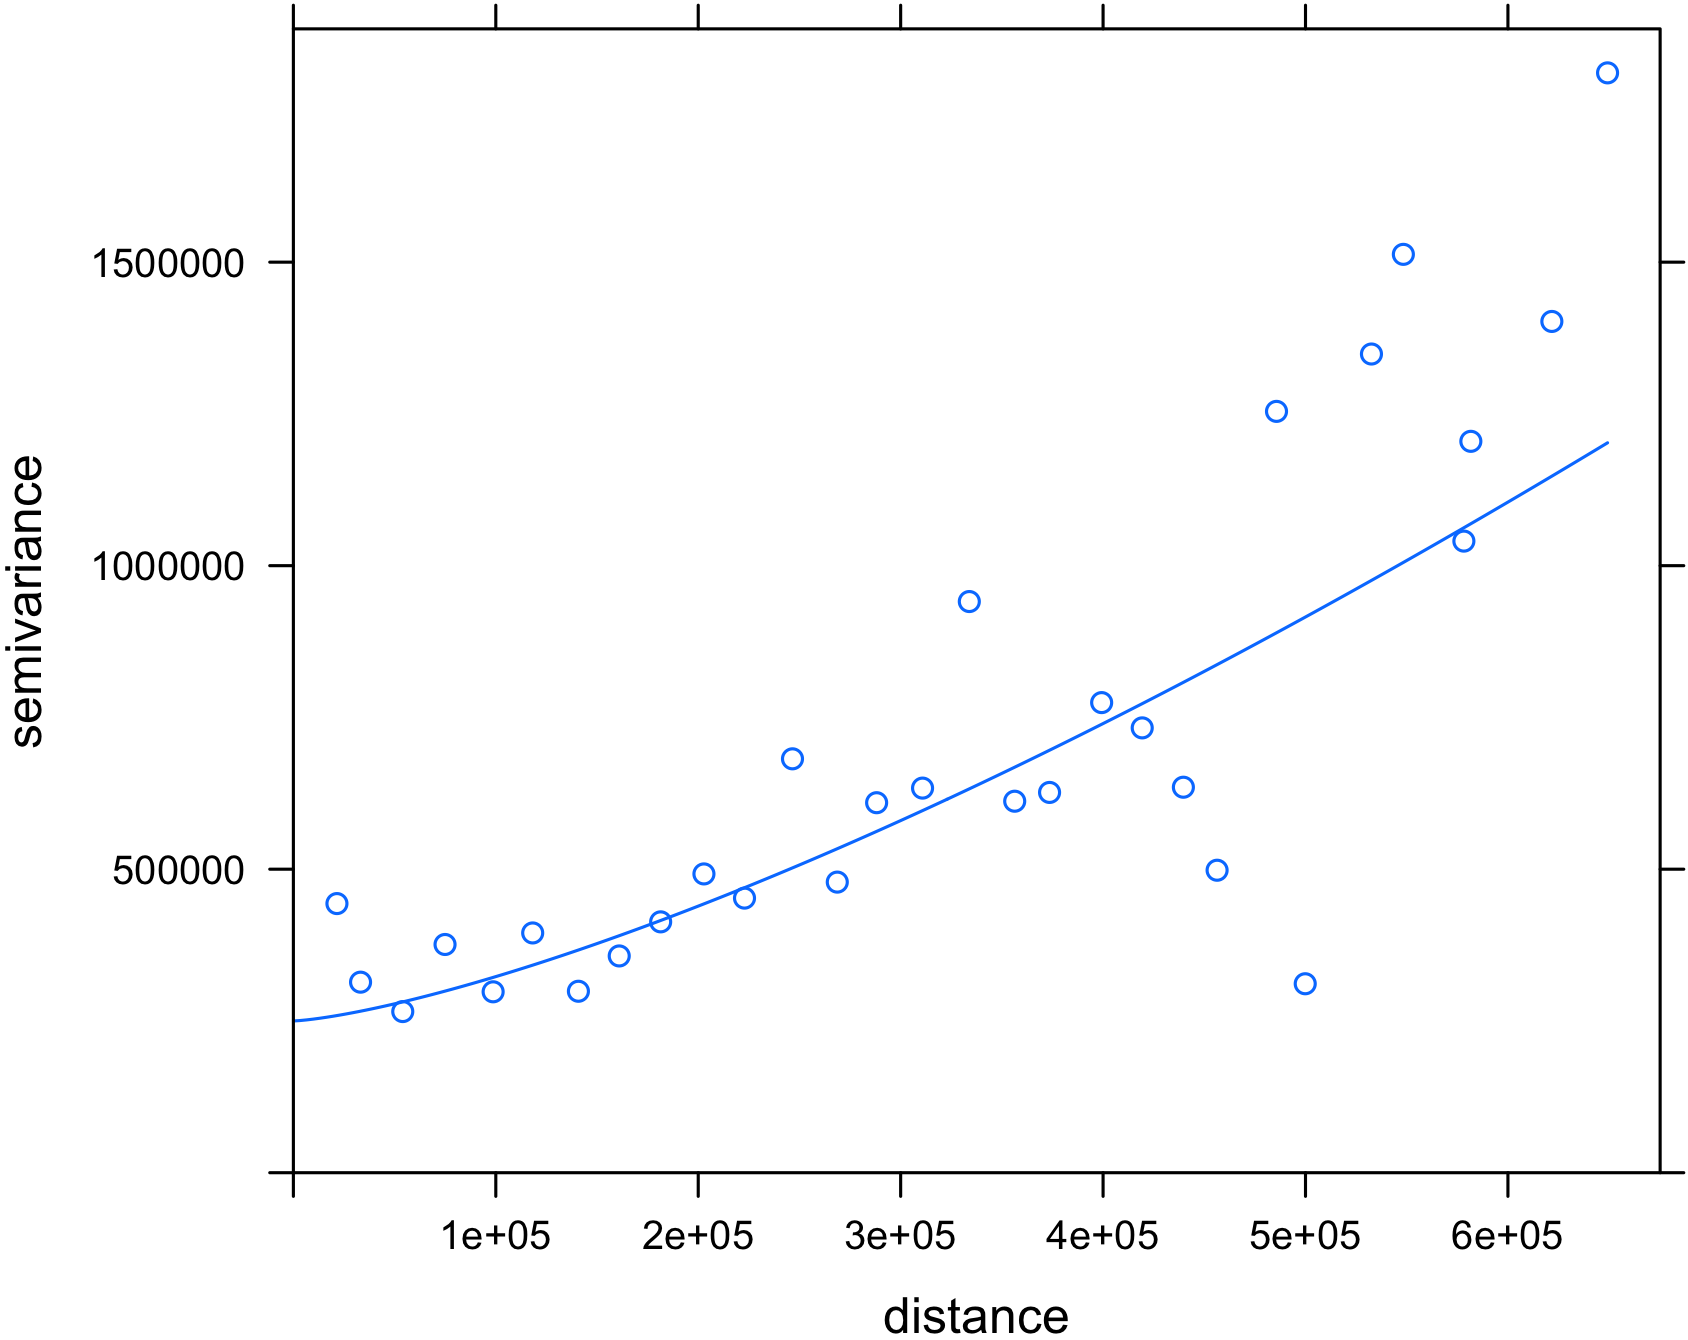
\includegraphics[width=1.15\textwidth]{images/SSTP7.png}
    \end{columns}\\
  \hspace{7cm} \footnotesize Wagner et al., 2012. J. Hydrol.}
    \only<4>
  {\begin{columns}
  \column{5cm}
    \centering
    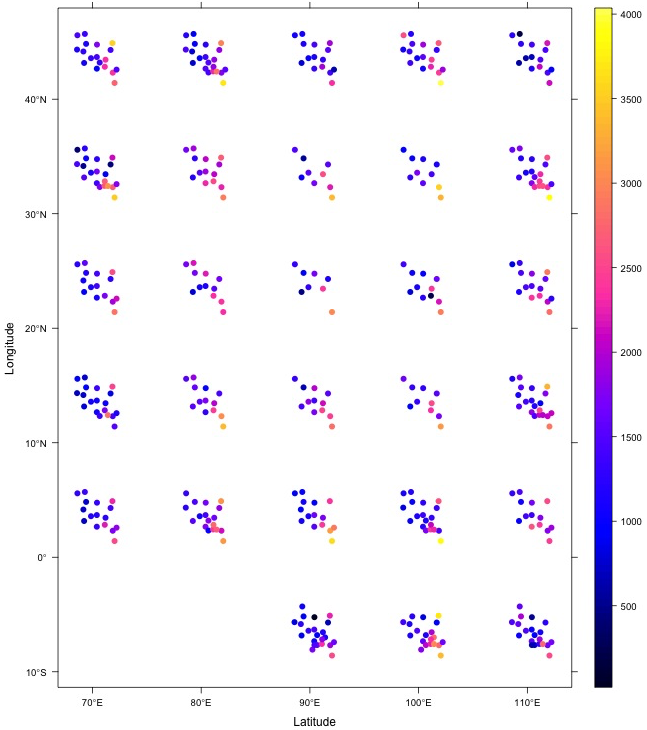
\includegraphics[width=1.15\textwidth]{images/SSTP5.png}
    \column{5cm}
    \centering
    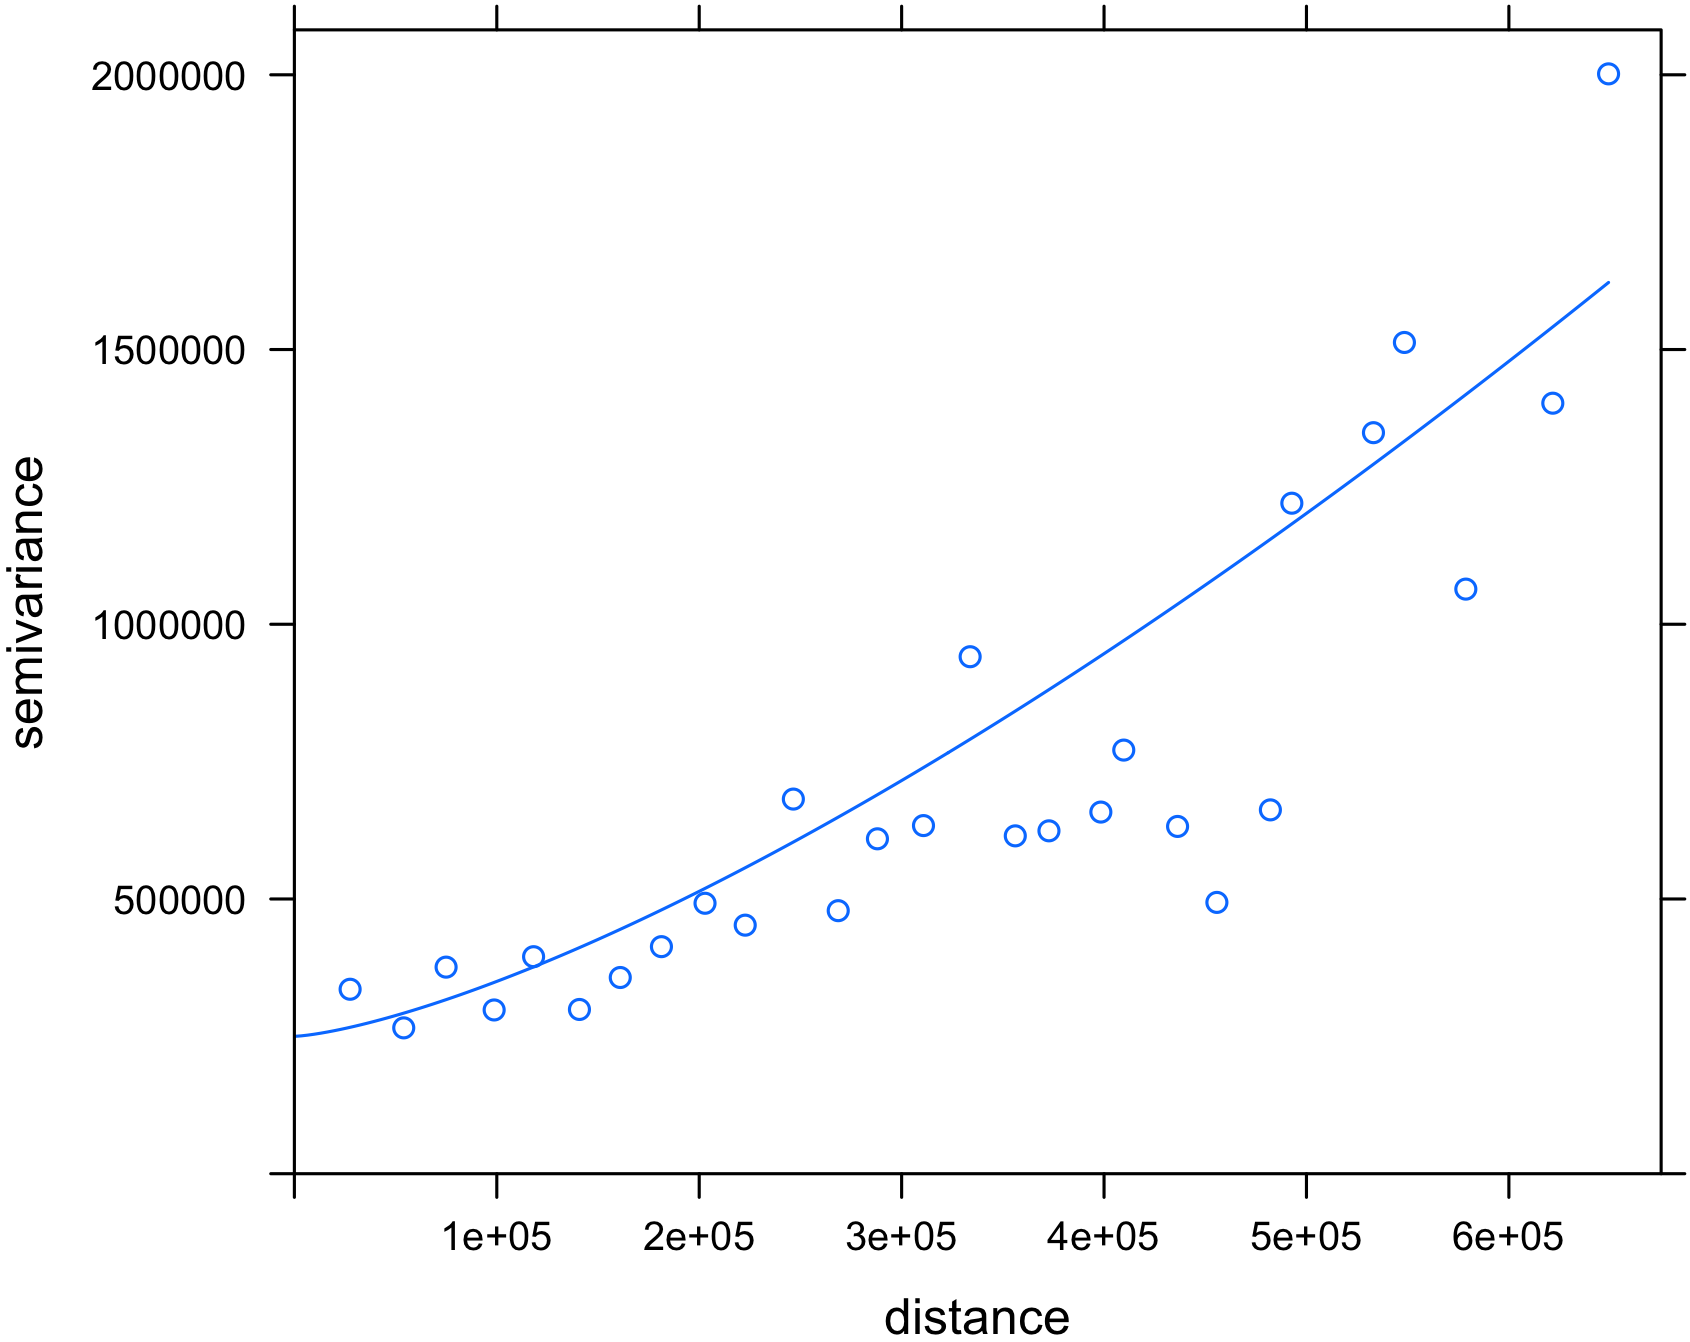
\includegraphics[width=1.15\textwidth]{images/SSTP8.png}
    \end{columns}}
\end{frame}

%%%%%%%%%%%%%%%%%%%%%%%%%%%%%%%%%%%%%%%%%%%%%%%%%%%%%%%%%%%%%

%%%%%%%%%%%%%%%%%%%%%%%%%%% Slide 12 %%%%%%%%%%%%%%%%%%%%%%%%%

\plain{}{\Large Climate response of aquatic insects\\\vspace{0.5cm}
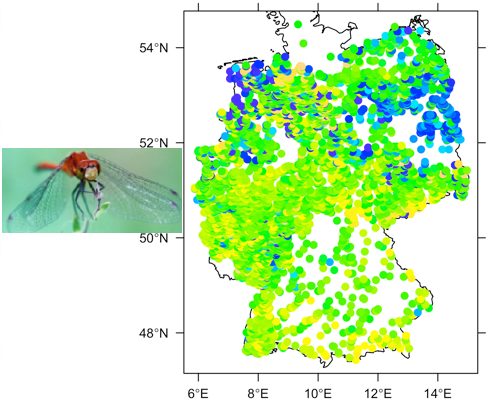
\includegraphics[width=0.68\textwidth]{images/St3.png}\\
\normalsize Bhowmik and Schäfer, 2015. PLOS ONE. e0130025}

%%%%%%%%%%%%%%%%%%%%%%%%%%% Slide 12 %%%%%%%%%%%%%%%%%%%%%%%%%

\begin{frame}
  \frametitle{Climate is the predominent driver \protect\\ of freshwater assemblages on large scales}
\centering
  $\vcenter{\hbox{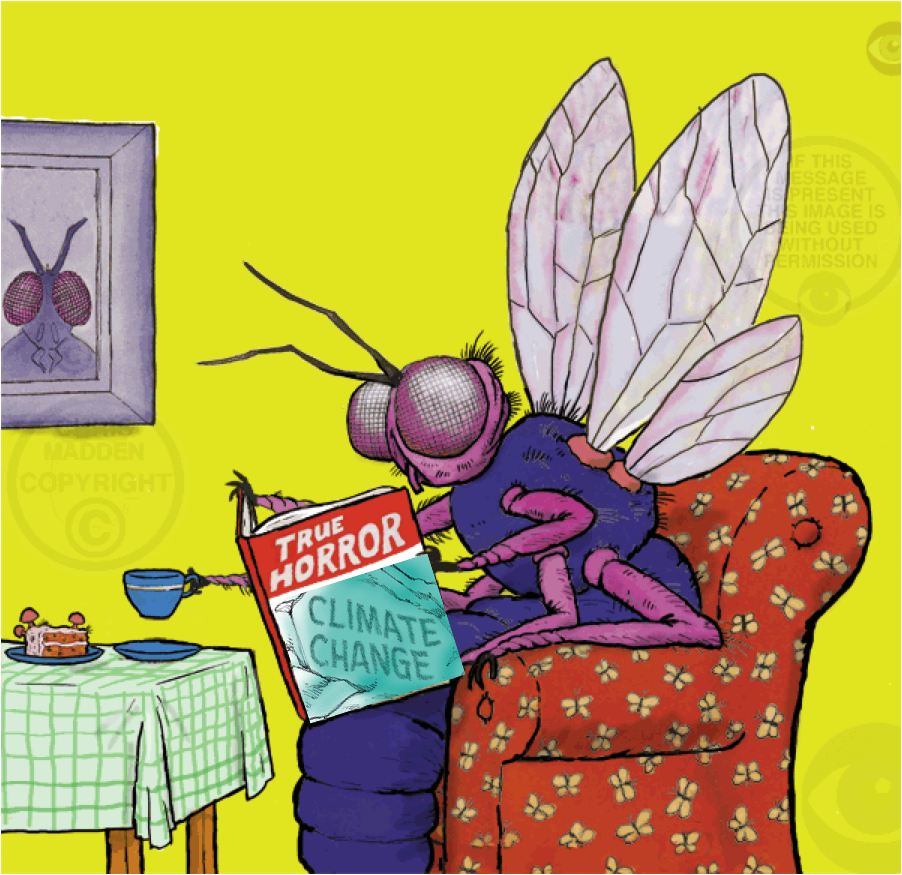
\includegraphics[width=0.4\textwidth]{images/Insect_Climate.png}}}$\\
  \pause
  \raggedright
  \vspace{10pt} \alert{Traits} are indicators of stressor effects in freshwater ecosystems \\
    \hspace{5.3cm} \footnotesize (Statzner and Bêche, 2010. Fresh. Bio.)\\
  \pause
  \normalsize \alert{Aquatic insects} disperse through landscape, not limited to streams\\
  \hspace{3cm} \footnotesize (Bonada et al., 2012. J. Biogeo.; Wikelski et al., 2006. Bio. Let.)\\
  \pause
 \normalsize \alert{Biological and ecological traits} were associated with climate change\\
  \raggedleft \hspace{3cm} \footnotesize (Hershkovitz et al., 2015. Eco. Ind.; Conti et al. 2013. Hydrobio.) 
\end{frame}

%%%%%%%%%%%%%%%%%%%%%%%%%%% Slide 13 %%%%%%%%%%%%%%%%%%%%%%%%%

\begin{frame}[fragile]
  \frametitle{Our research questions \protect\\ were two-fold}
  \begin{enumerate}
  \item which climate-associated traits and organism groups show the highest potential for changing distribution pattern?
  \medskip
  \pause
  \item which are most influential climatic aspects for traits and organism groups showing highest potential for changing distribution?
  \end{enumerate}
\end{frame}

%%%%%%%%%%%%%%%%%%%%%%%%%%% Slide 14 %%%%%%%%%%%%%%%%%%%%%%%%%

\begin{frame}
  \frametitle{Biomonitoring data from 4,752 stream sites \protect\\ and 35 global bioclimatic indices }
  $\vcenter{\hbox{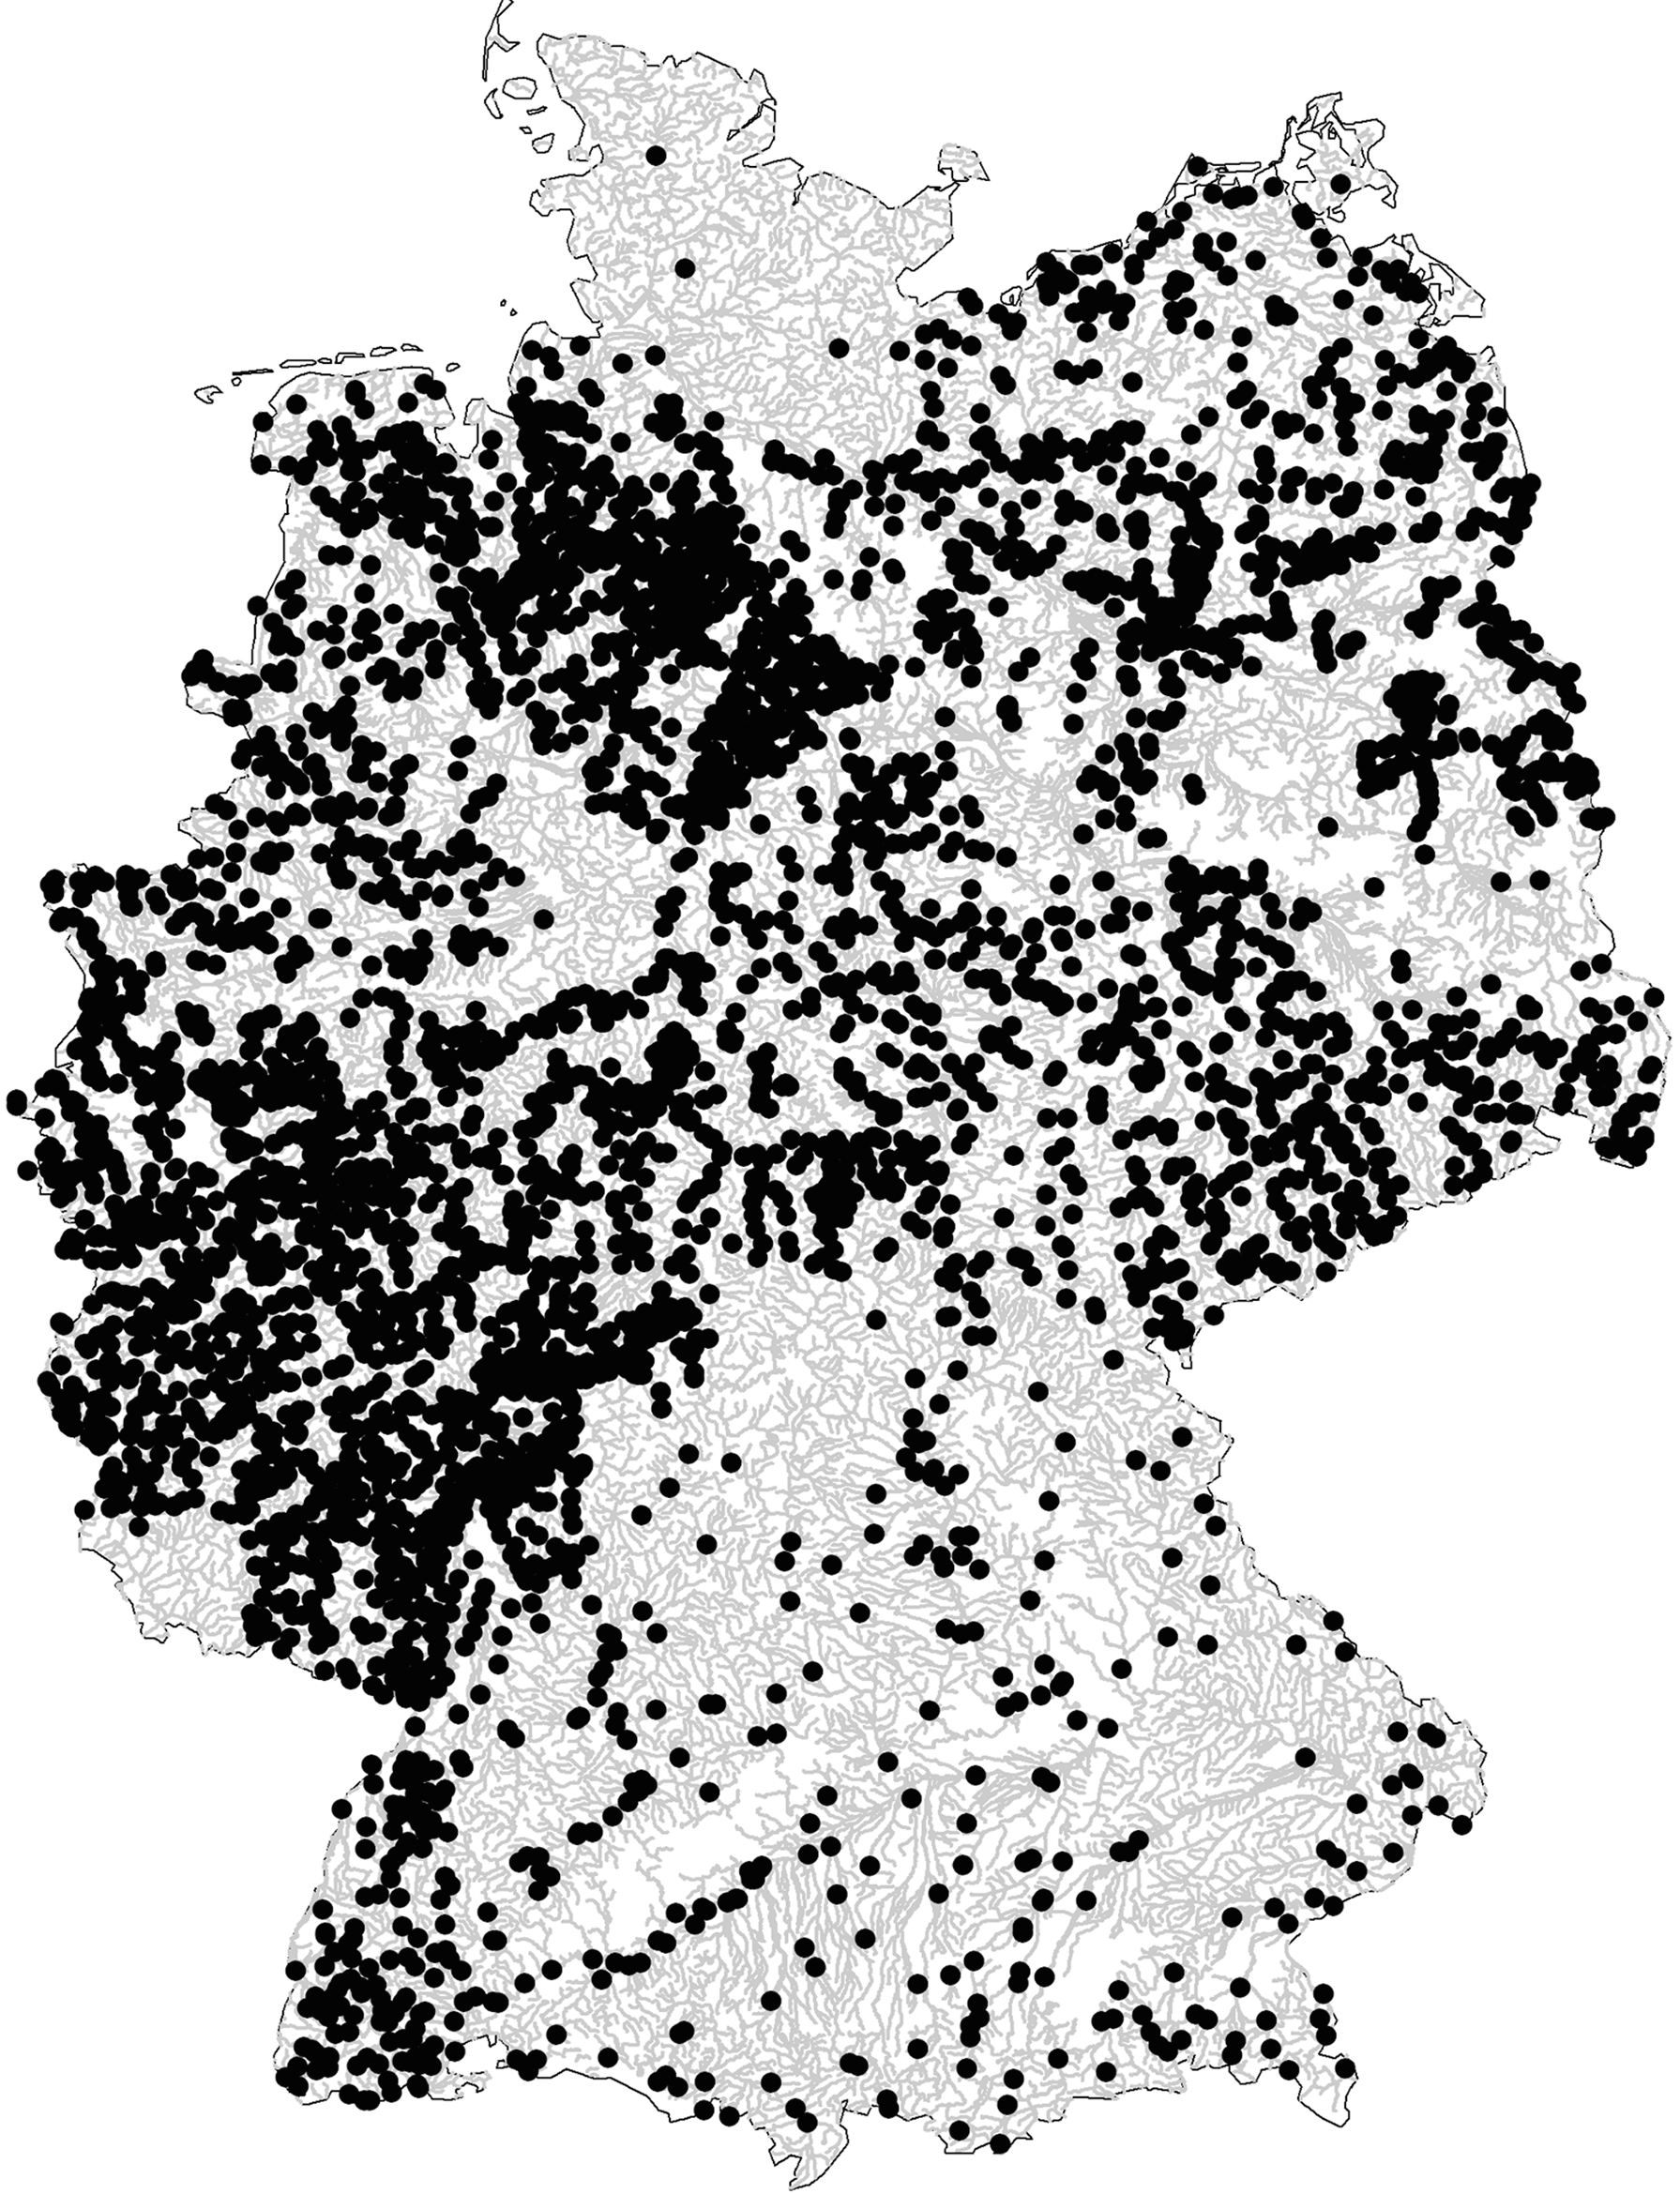
\includegraphics[width=0.46\textwidth]{images/Germany_Sites.png}}}$
  \hspace{0.2cm}
  $\vcenter{\hbox{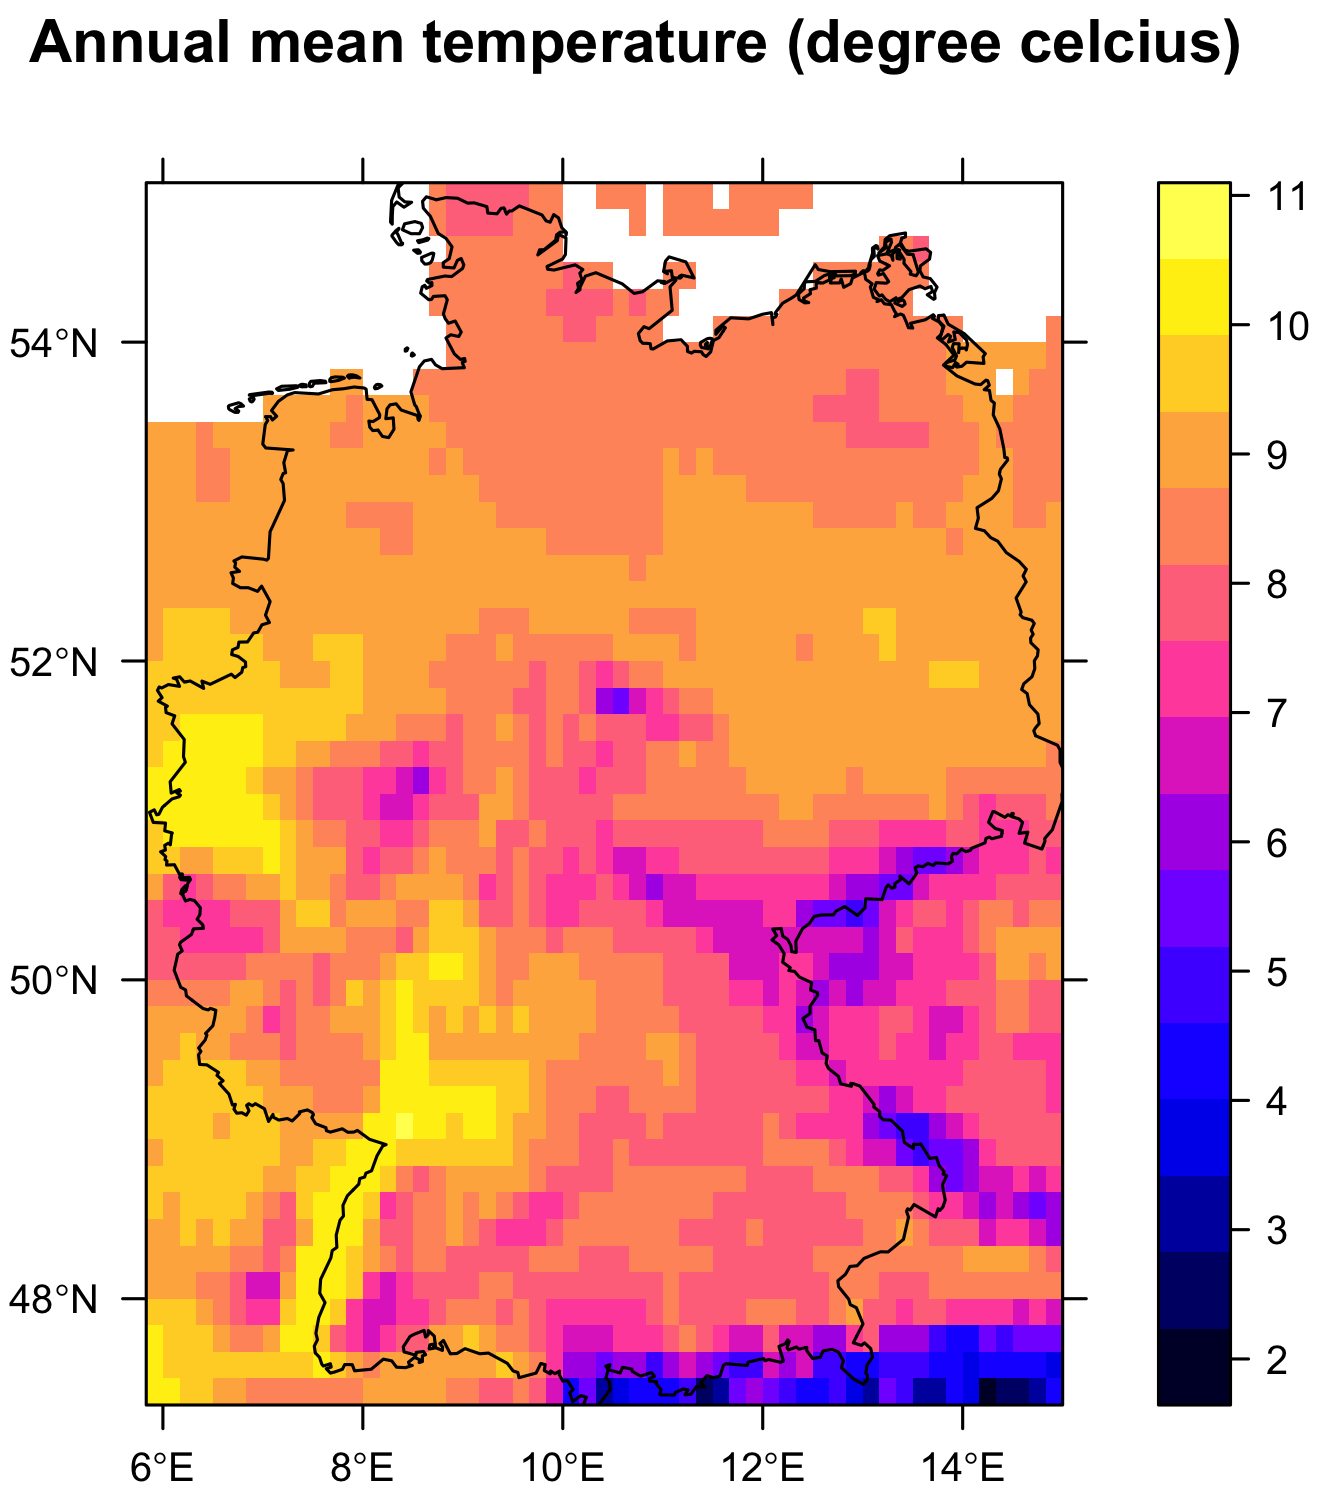
\includegraphics[width=0.48\textwidth]{images/Bioclim.png}}}$ \\
  \hspace{45pt} \alert{357,000 km\textsuperscript{2}} \hspace{110pt} \alert{18 km}\\
  \hspace{5cm} \footnotesize Biss et al., 2006; Kriticos et al., 2012. Met. Eco. Evo.
\end{frame}

%%%%%%%%%%%%%%%%%%%%%%%%%%% Slide 15 %%%%%%%%%%%%%%%%%%%%%%%%%

\begin{frame}[fragile]
  \frametitle{Climate-associated traits \protect\\ from 6 grouping features and 5 aquatic insect orders}

  \centering
  $\vcenter{\hbox{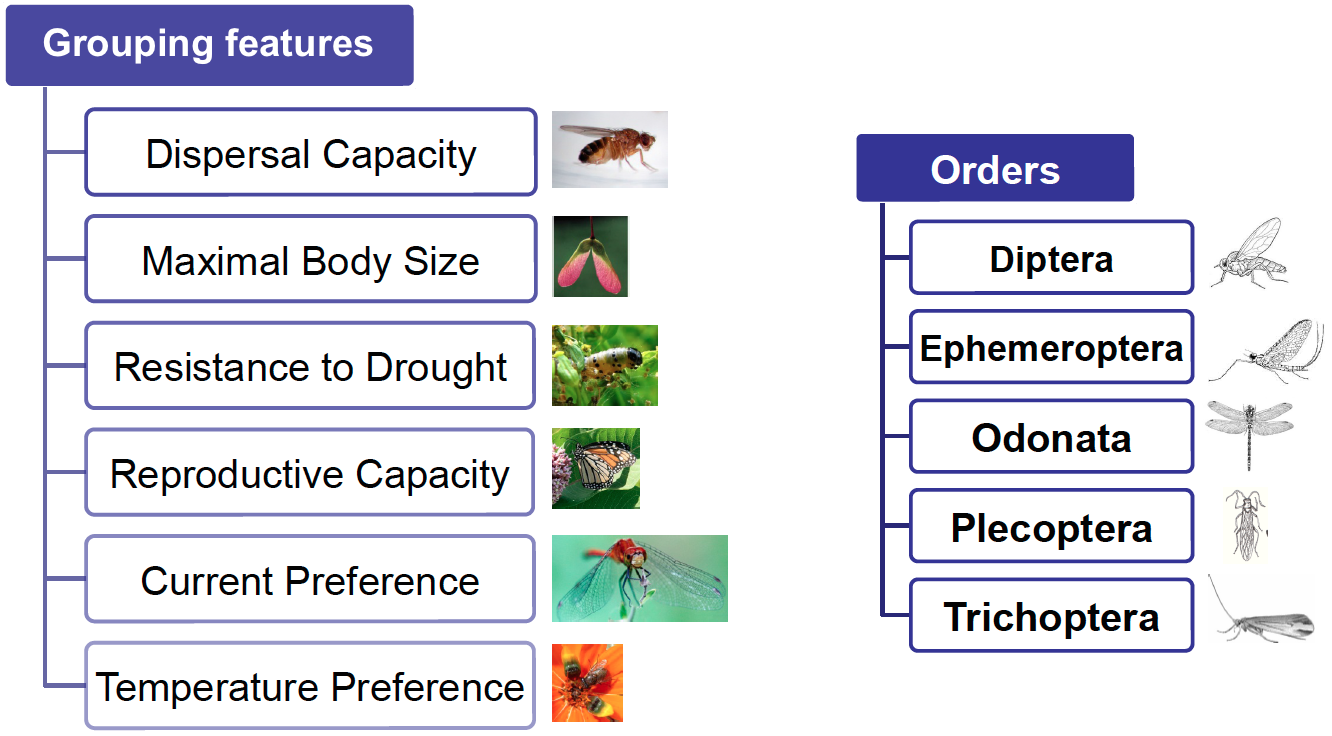
\includegraphics[width=1\textwidth]{images/Traits_Orders.png}}}$\\
    \vspace{10pt} Trait databases: \alert{freshwater ecology \footnotesize (Schmidt-Kloiber and Hering, 2015), \normalsize Tachet \footnotesize (Usseglio-Polatera et al. 2000)}\\
\end{frame}

%%%%%%%%%%%%%%%%%%%%%%%%%%% Slide 16 %%%%%%%%%%%%%%%%%%%%%%%%%

\begin{frame}[fragile]
  \frametitle{We linked biomonitoring data with trait data\protect\\ and computed abundance-weighted traits \footnotesize}
  \pause
  \centering
  $\vcenter{\hbox{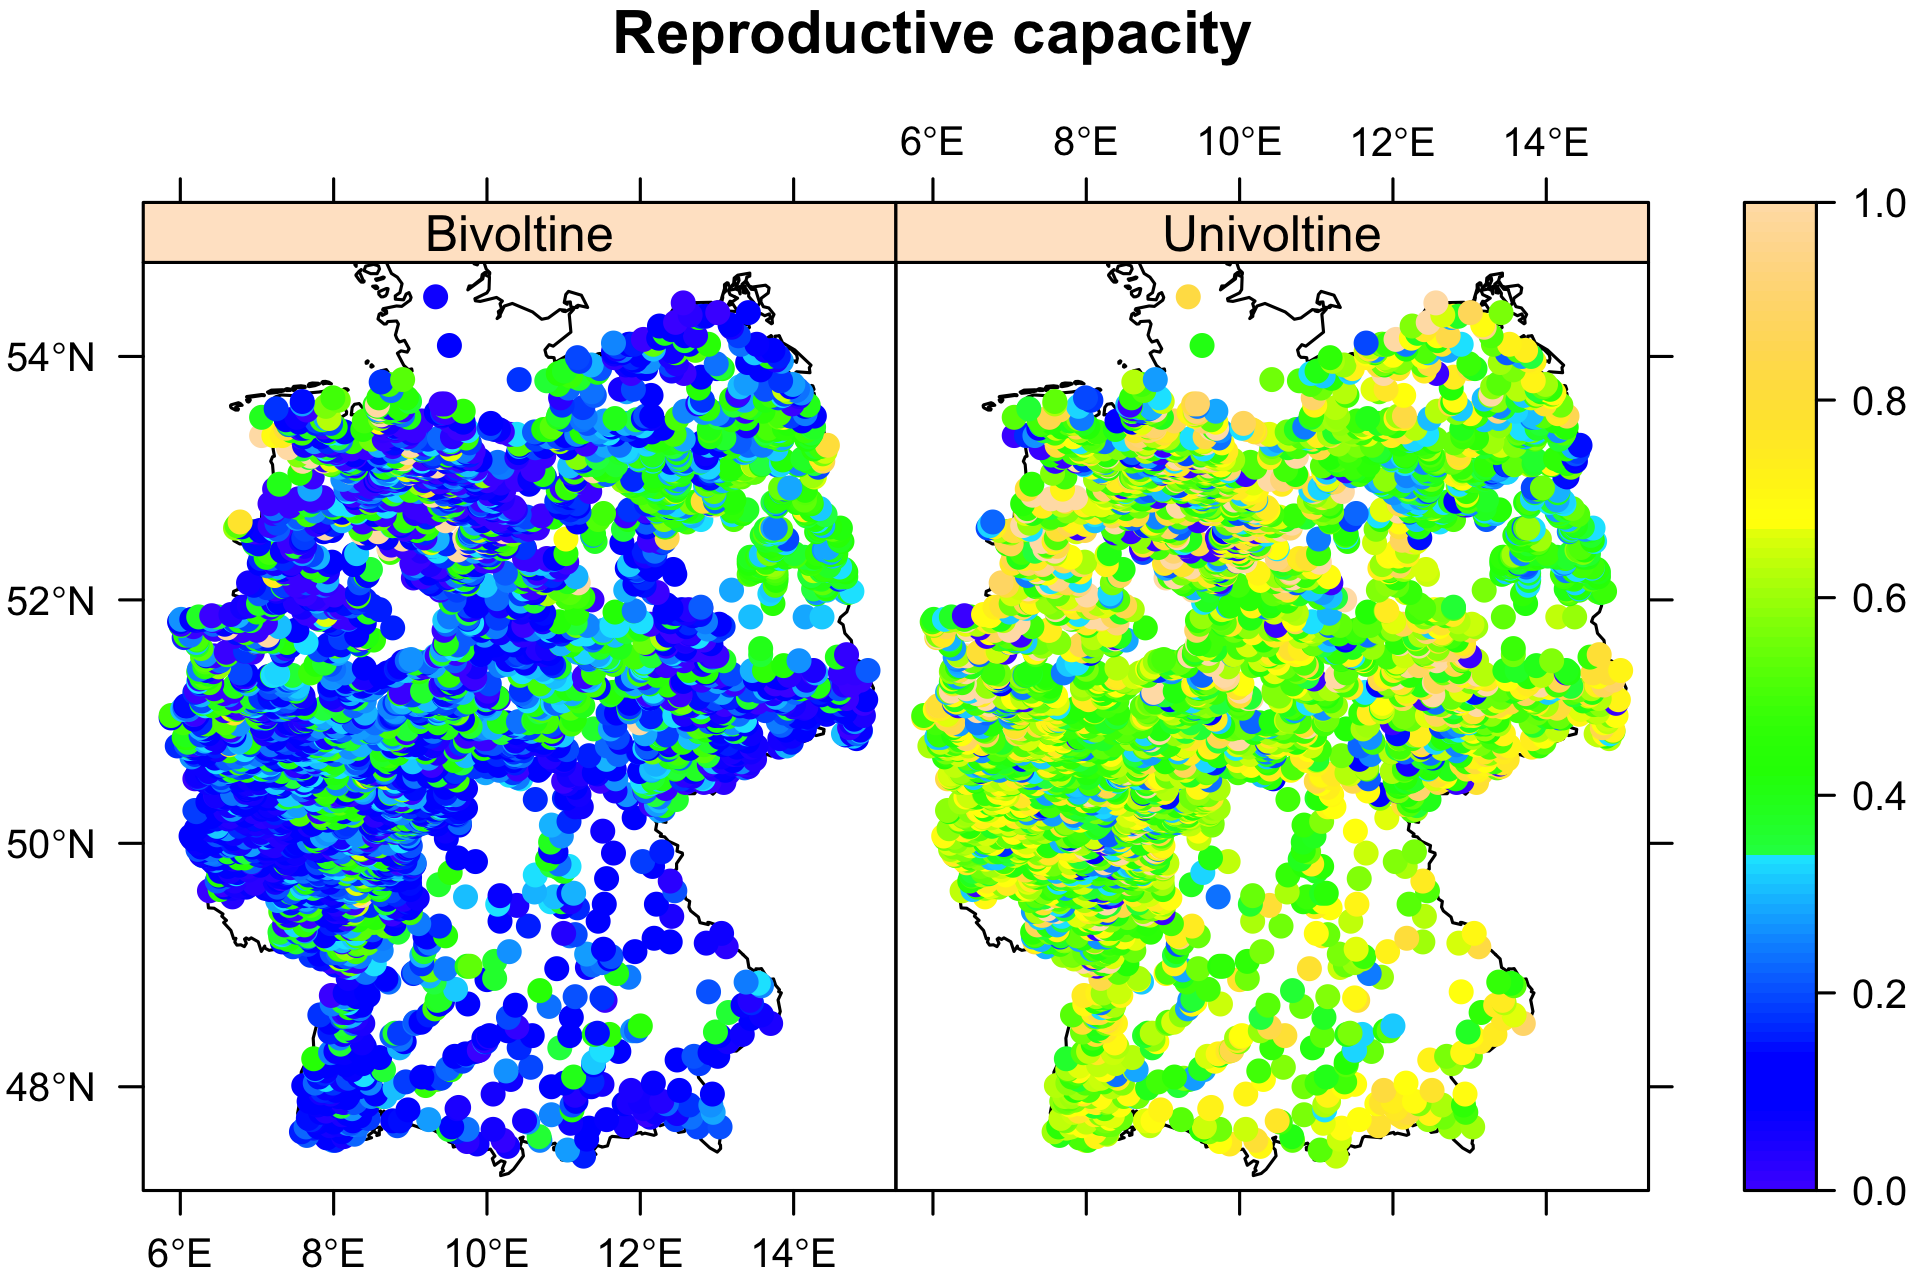
\includegraphics[width=0.95\textwidth]{images/Reprocapa.png}}}$\\ \\
  \hspace{6cm} \footnotesize Schmera et al. 2014. Fresh. Bio.
\end{frame}

%%%%%%%%%%%%%%%%%%%%%%%%%%% Slide 17 %%%%%%%%%%%%%%%%%%%%%%%%%

\begin{frame}[fragile]
  \frametitle{We quantified the amount of spatial autocorrelation\protect\\ that is associated with bioclimatic indices}
  \begin{enumerate}
  \item Spatial autocorrelation \alert{(Global Moran's I)} in abundance-weighted traits\\
  \pause
  \alert{\small Spatial autocorrelation measures strength of spatial pattern in the distribution of traits \footnotesize (Dray et al. 2012. Eco. Mono.)}\\
  \pause
  \item \alert{Trait-Climate model:} relationship between abundance-weighted traits and bioclimatic indices
  \pause
  \item Global Moran's I in the residuals of trait-climate model
  \pause
  \item Relationship between abundance-weighted traits and individual bioclimatic indices
  \end{enumerate} 
\end{frame}

%%%%%%%%%%%%%%%%%%%%%%%%%%% Slide 18 %%%%%%%%%%%%%%%%%%%%%%%%%

\begin{frame}[fragile]
  \frametitle{59 \% spatial autocorrelation in abundance-weighted traits\protect\\was associated with bioclimatic indices}
  \pause
  Highest spatial autocorrelation was explained:
  \begin{itemize}
  \item in \alert{temperature preference (81 \%)} , particularly in insects with \alert{cold temperature preference (91 \%)} $\vcenter{\hbox{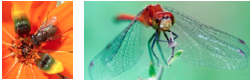
\includegraphics[width=0.15\textwidth]{images/Temperature.png}}}$
  \medskip
  \pause
  \item for \alert{Ephemeroptera (59 \%)}, particularly for \alert{Trichoptera with moderate temperature preference (97 \%)}  $\vcenter{\hbox{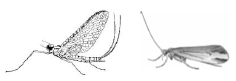
\includegraphics[width=0.15\textwidth]{images/Orders.png}}}$
  \medskip
  \pause
  \item Traits of \alert{temperature preference} showed strong covariation with underlying \alert{climate-associated traits} %\\
  %\pause
  %e.g. \alert{low dispersal capacity, large body size (>4 cm), low reproductive capacity (semivoltine) and resistance to drought (egg diapause) together explained 55 \% of cold temperature preference}
  \end{itemize}
\end{frame}

%%%%%%%%%%%%%%%%%%%%%%%%%%% Slide 19 %%%%%%%%%%%%%%%%%%%%%%%%%

\begin{frame}[fragile]
  \frametitle{59 \% spatial autocorrelation in abundance-weighted traits\protect\\was associated with bioclimatic indices}
  \centering
  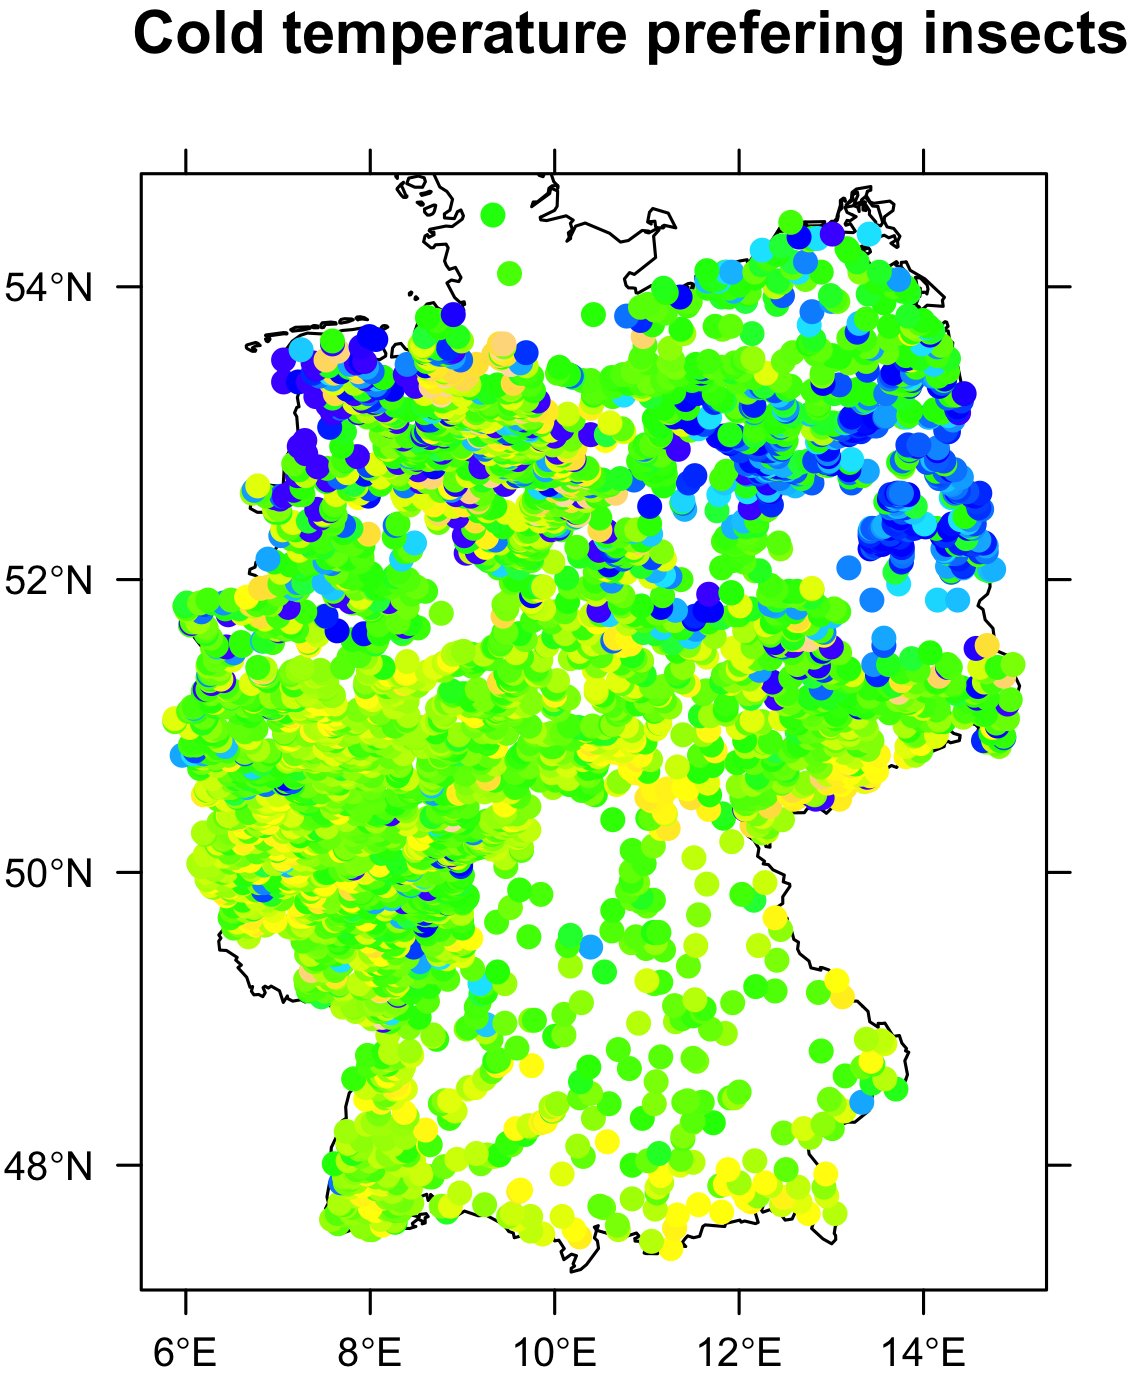
\includegraphics[width=0.45\textwidth]{images/Cold.png}
  \pause
  \hspace{2pt}
  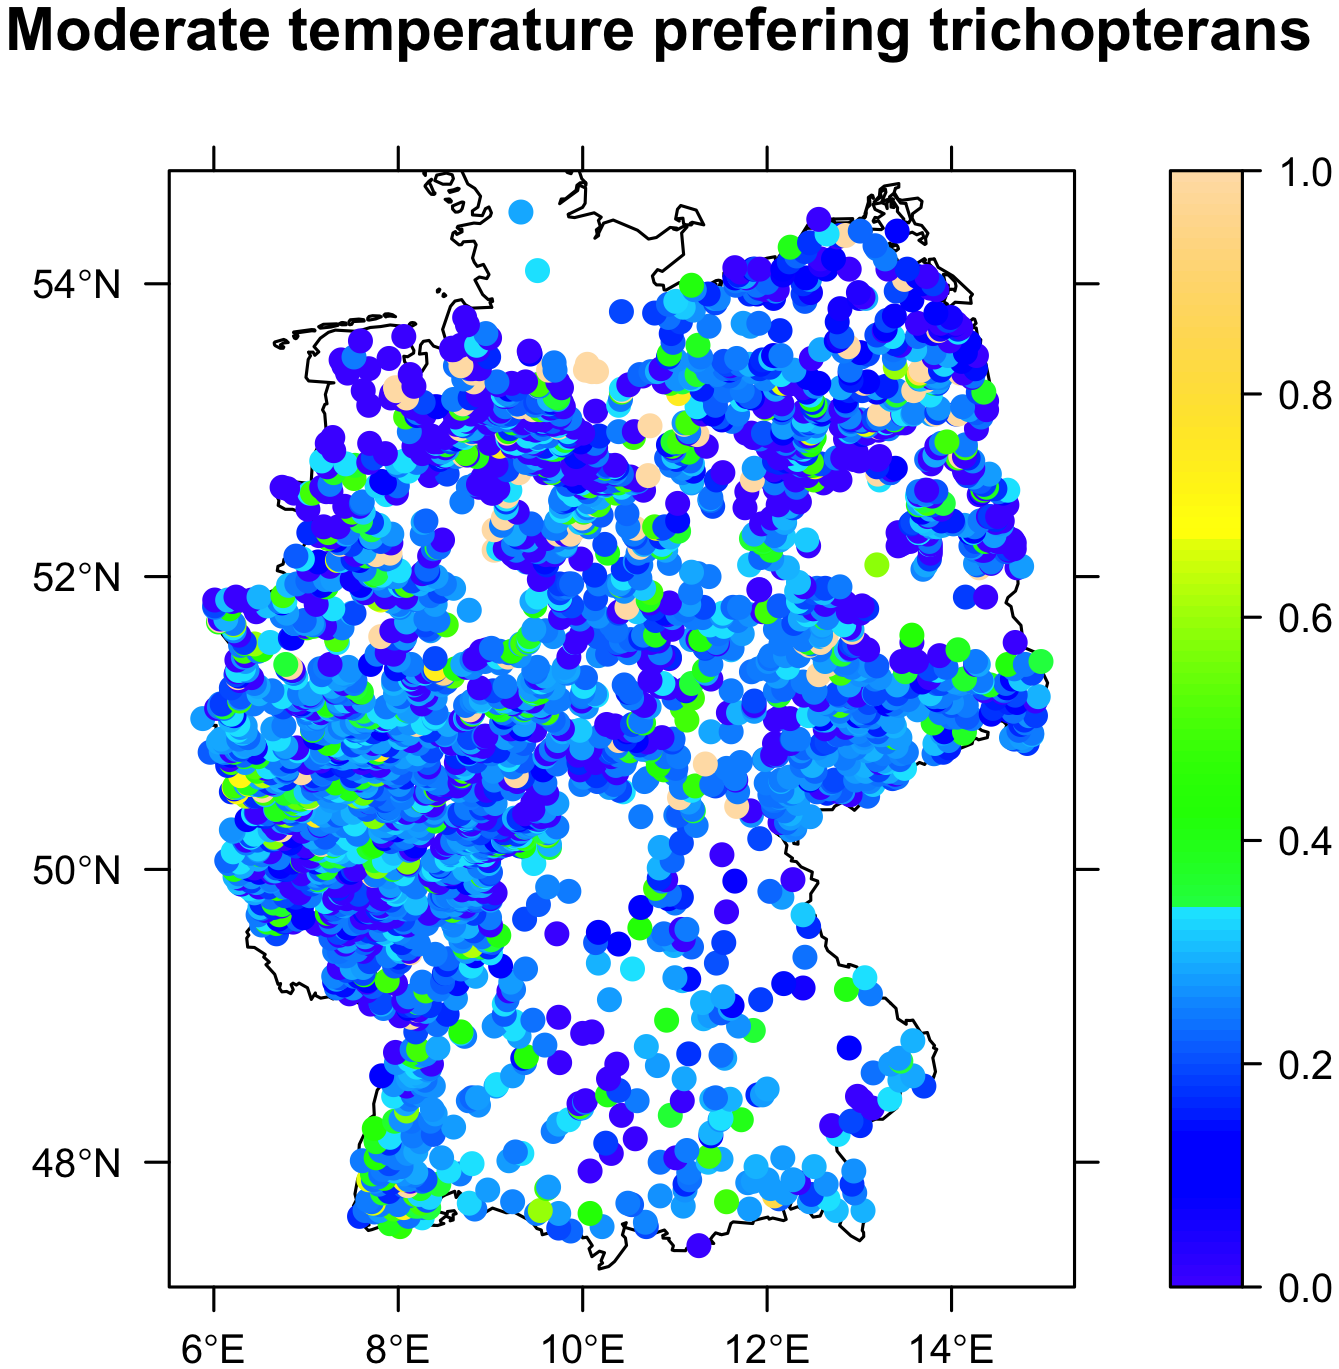
\includegraphics[width=0.535\textwidth]{images/Modetri.png}
\end{frame}

%%%%%%%%%%%%%%%%%%%%%%%%%%% Slide 20 %%%%%%%%%%%%%%%%%%%%%%%%%

\begin{frame}[fragile]
\frametitle{Seasonal radiation and temperature\protect\\were the most influential bioclimatic aspects}
\begin{itemize}
\item \alert{Radiation seasonality (46 \%)} explained highest spatial autocorrelation in cold temperature preferring insects
\pause
\item \alert{Radiation (65 \%) and mean temperature (64 \%) of the driest quarter} explained highest spatial autocorrelation in moderate temperature preferring trichopterans
\end{itemize}
\pause
\centering
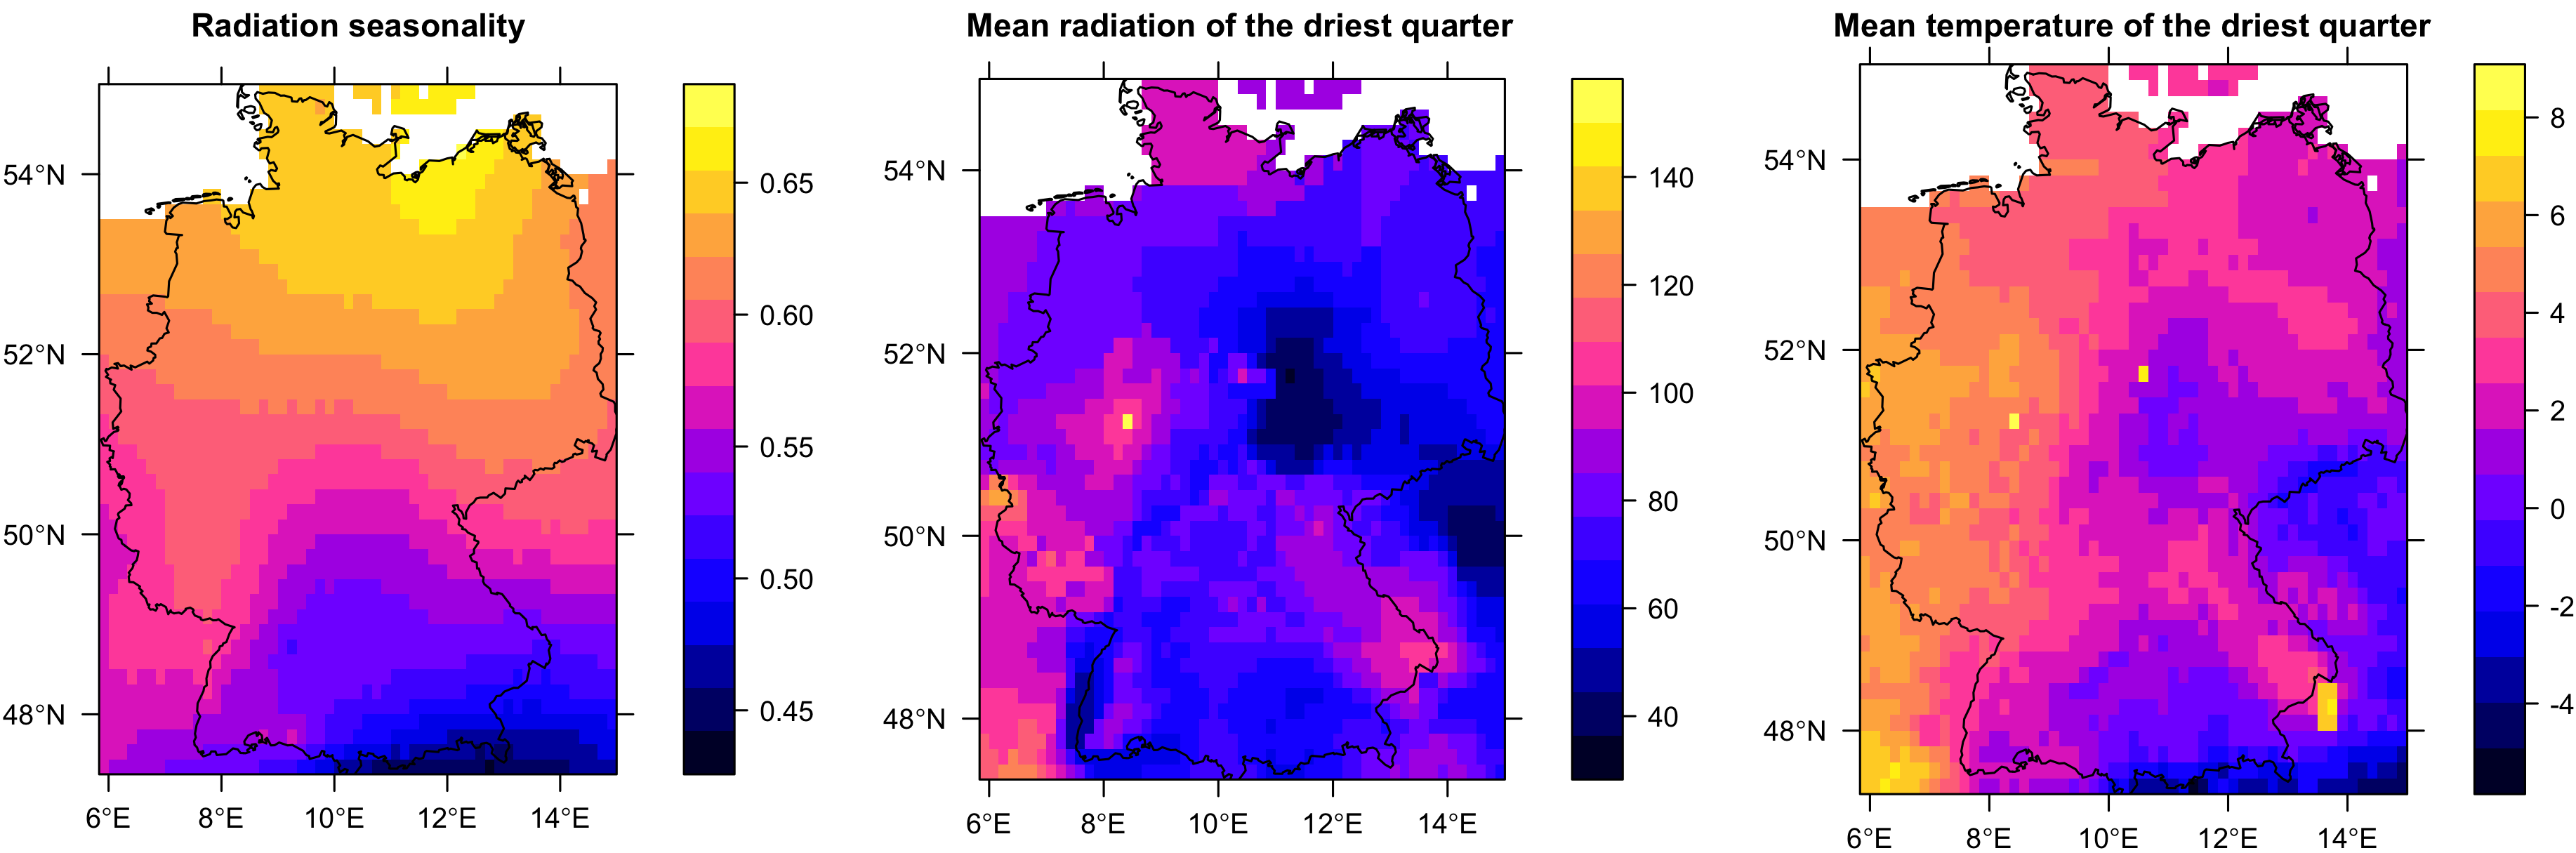
\includegraphics[width=1\textwidth]{images/Inf_Bio.png}
\end{frame}

%%%%%%%%%%%%%%%%%%%%%%%%%%% Slide 21 %%%%%%%%%%%%%%%%%%%%%%%%%

\begin{frame}{We anticipate change in aquatic insect distribution pattern\protect\\ along the longitudinal gradient in Germany}
\begin{itemize}
\item \alert{Winter and summer temperature may increase in the South} \footnotesize{(Stocker et al. 2013. IPCC report)}
\pause
\item \normalsize \alert{Cold temperature preferring insects} mostly occur in the South\\
\pause
\vspace{10pt}
\begin{itemize}
\item insects with low dispersal capacity \footnotesize{(Hershkovitz et al. 2015. Eco. Ind.)}\\
\pause
\vspace{10pt}
\item \normalsize large-bodied insects \footnotesize{(Harrison et al., 2010. Bio. Sci.)}\\
\pause
\vspace{10pt}
\item \normalsize \alert{hence, may shrink their distribution} \footnotesize (Verberk and Atkinson, 2013. Func. Eco.)
\end{itemize}
\pause
\medskip
\item \normalsize \alert{Moderate temperature preferring trichopterans} mostly occur in the North may extend their range \footnotesize{(Hering et al. 2009. Aq. Sci.)}
\end{itemize}
\end{frame}

%%%%%%%%%%%%%%%%%%%%%%%%%%% Slide 22 %%%%%%%%%%%%%%%%%%%%%%%%%

\begin{frame}{Adaptation may occur and\protect\\agglomerate ecological effects}
\begin{columns}
\column{7cm}
\begin{itemize}
\item \alert{Trait evolution} \footnotesize (Lancaster and Downes, 2010. Riv. Res. App.) \normalsize\\
\vspace{0.5cm}
\item \alert{Trait adaptation} \footnotesize Zeuss et al., 2014. Nat. Com.
\end{itemize}
\column{4cm}
\centering

\includegraphics[width=1.1\textwidth]{images/Brave.png}
\end{columns}
\end{frame}

%%%%%%%%%%%%%%%%%%%%%%%%%%%%%%%%%%%%%%%%%%%%%%%%%%%%%%%%%%%%%

%%%%%%%%%%%%%%%%%%%%%%%%%%% Slide 23 %%%%%%%%%%%%%%%%%%%%%%%%%

\plain{}{\Large Human health risks from trace metals\\\vspace{0.5cm}
\includegraphics[width=0.7\textwidth]{images/St4.png}\\
\normalsize Bhowmik et al. 2015. Sci. Tot. Env. 538: 306-316}

%%%%%%%%%%%%%%%%%%%%%%%%%%% Slide 24 %%%%%%%%%%%%%%%%%%%%%%%%%

\begin{frame}%[fragile]
  \frametitle{1/3 of annual mortality in Pakistan \protect\\ is attributed to contaminated drinking water}
  \onslide<1-> {$\vcenter{\hbox{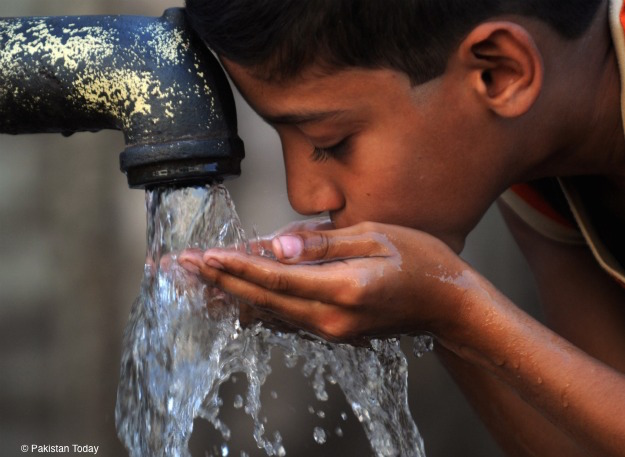
\includegraphics[width=0.32\textwidth]{images/Water_Pakistan.jpg}}}$}
  \onslide<2-> {\hspace*{10pt}
    $\vcenter{\hbox{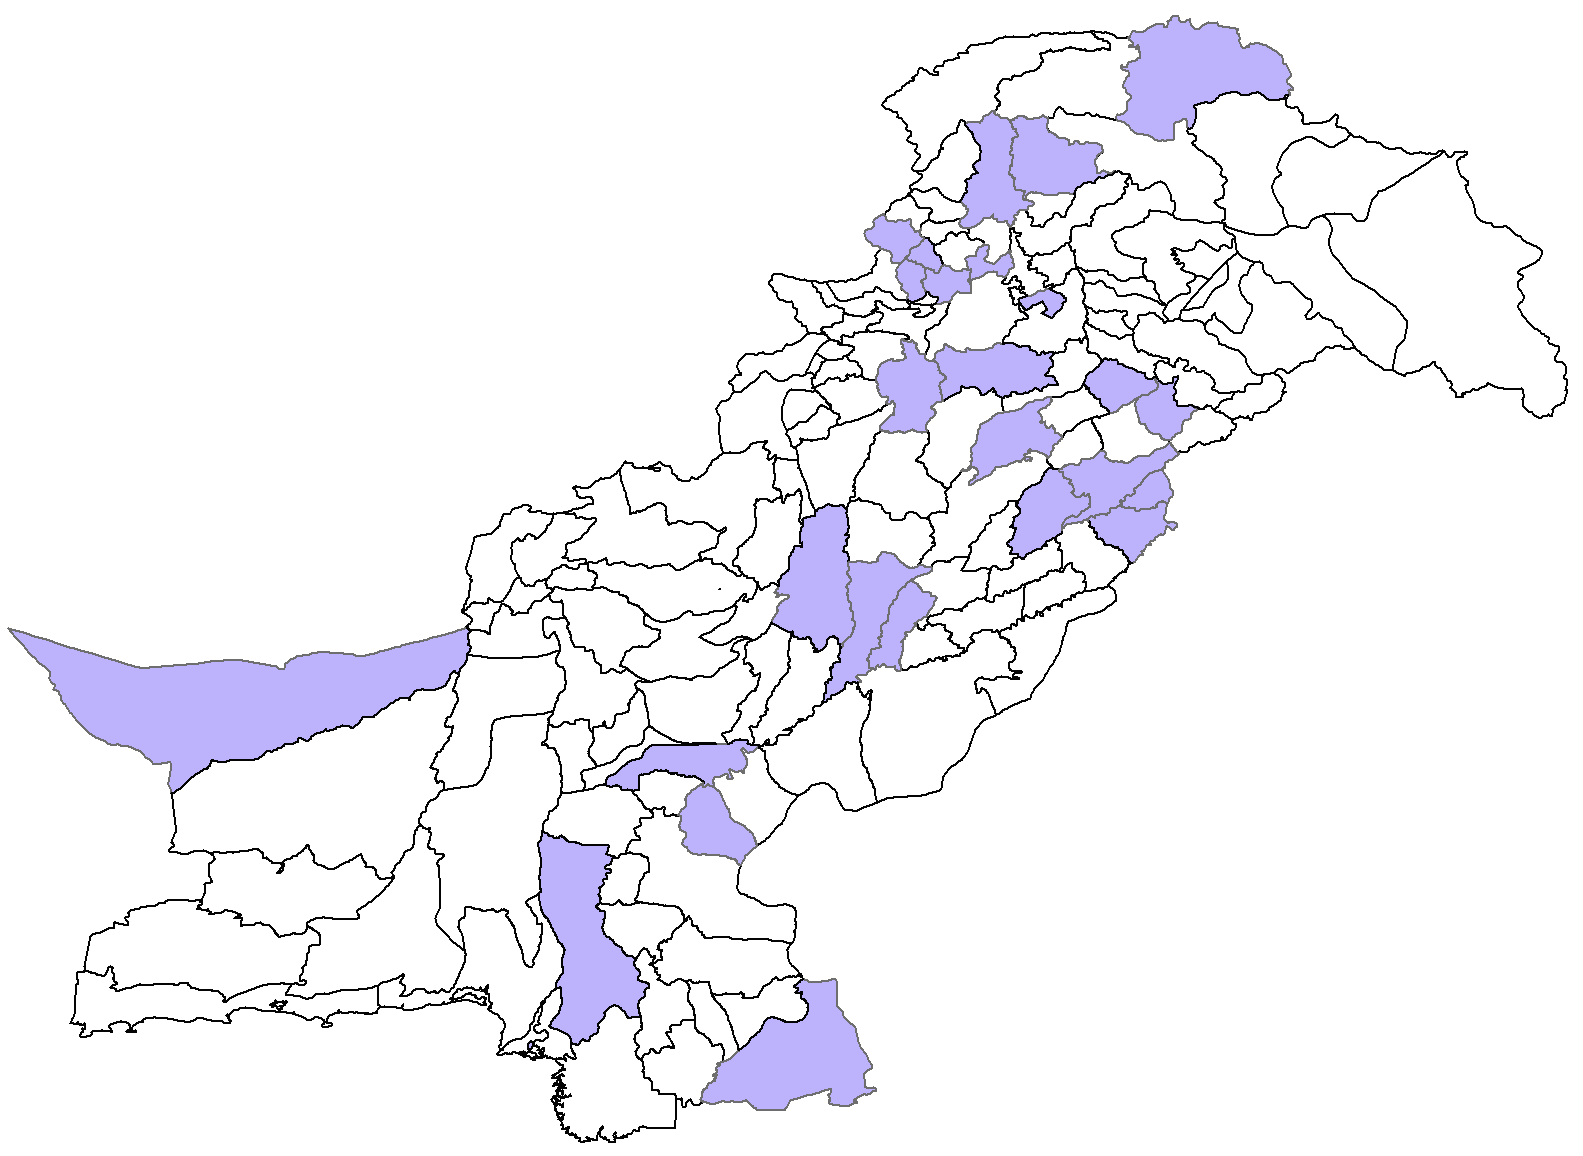
\includegraphics[width=0.62\textwidth]{images/Districts_Pakistan.png}}}$ \\}
  \onslide<1-> {\footnotesize Azizullah et al. 2011. Env. Int.\normalsize\\ \\}
  \onslide<3-> {\alert{We compiled trace metal concentrations in ground \& surface water} \\}
  \onslide<4-> {19\% coverage, max. sampled-unsampled district distance 2000 km \\}
  \onslide<5> {Low global representativeness, GCV $\geq$ 1, \alert{non-stationarity}}
\end{frame}

%%%%%%%%%%%%%%%%%%%%%%%%%%% Slide 25 %%%%%%%%%%%%%%%%%%%%%%%%%

\begin{frame}
  \frametitle{Geographically weighted regression (GWR) \protect\\ allows to incorporate local variations}
  \vspace{-15pt}
  \begin{equation*}
    C_{T,z} = \delta_{z,0} + \sum_{n=1}^{m=8}\delta_{z,n}S_{z,n} + e_z
    \end{equation*}\\
    \footnotesize Harris et al. 2010. Math. Geosci.\\ \\\normalsize
    \pause
    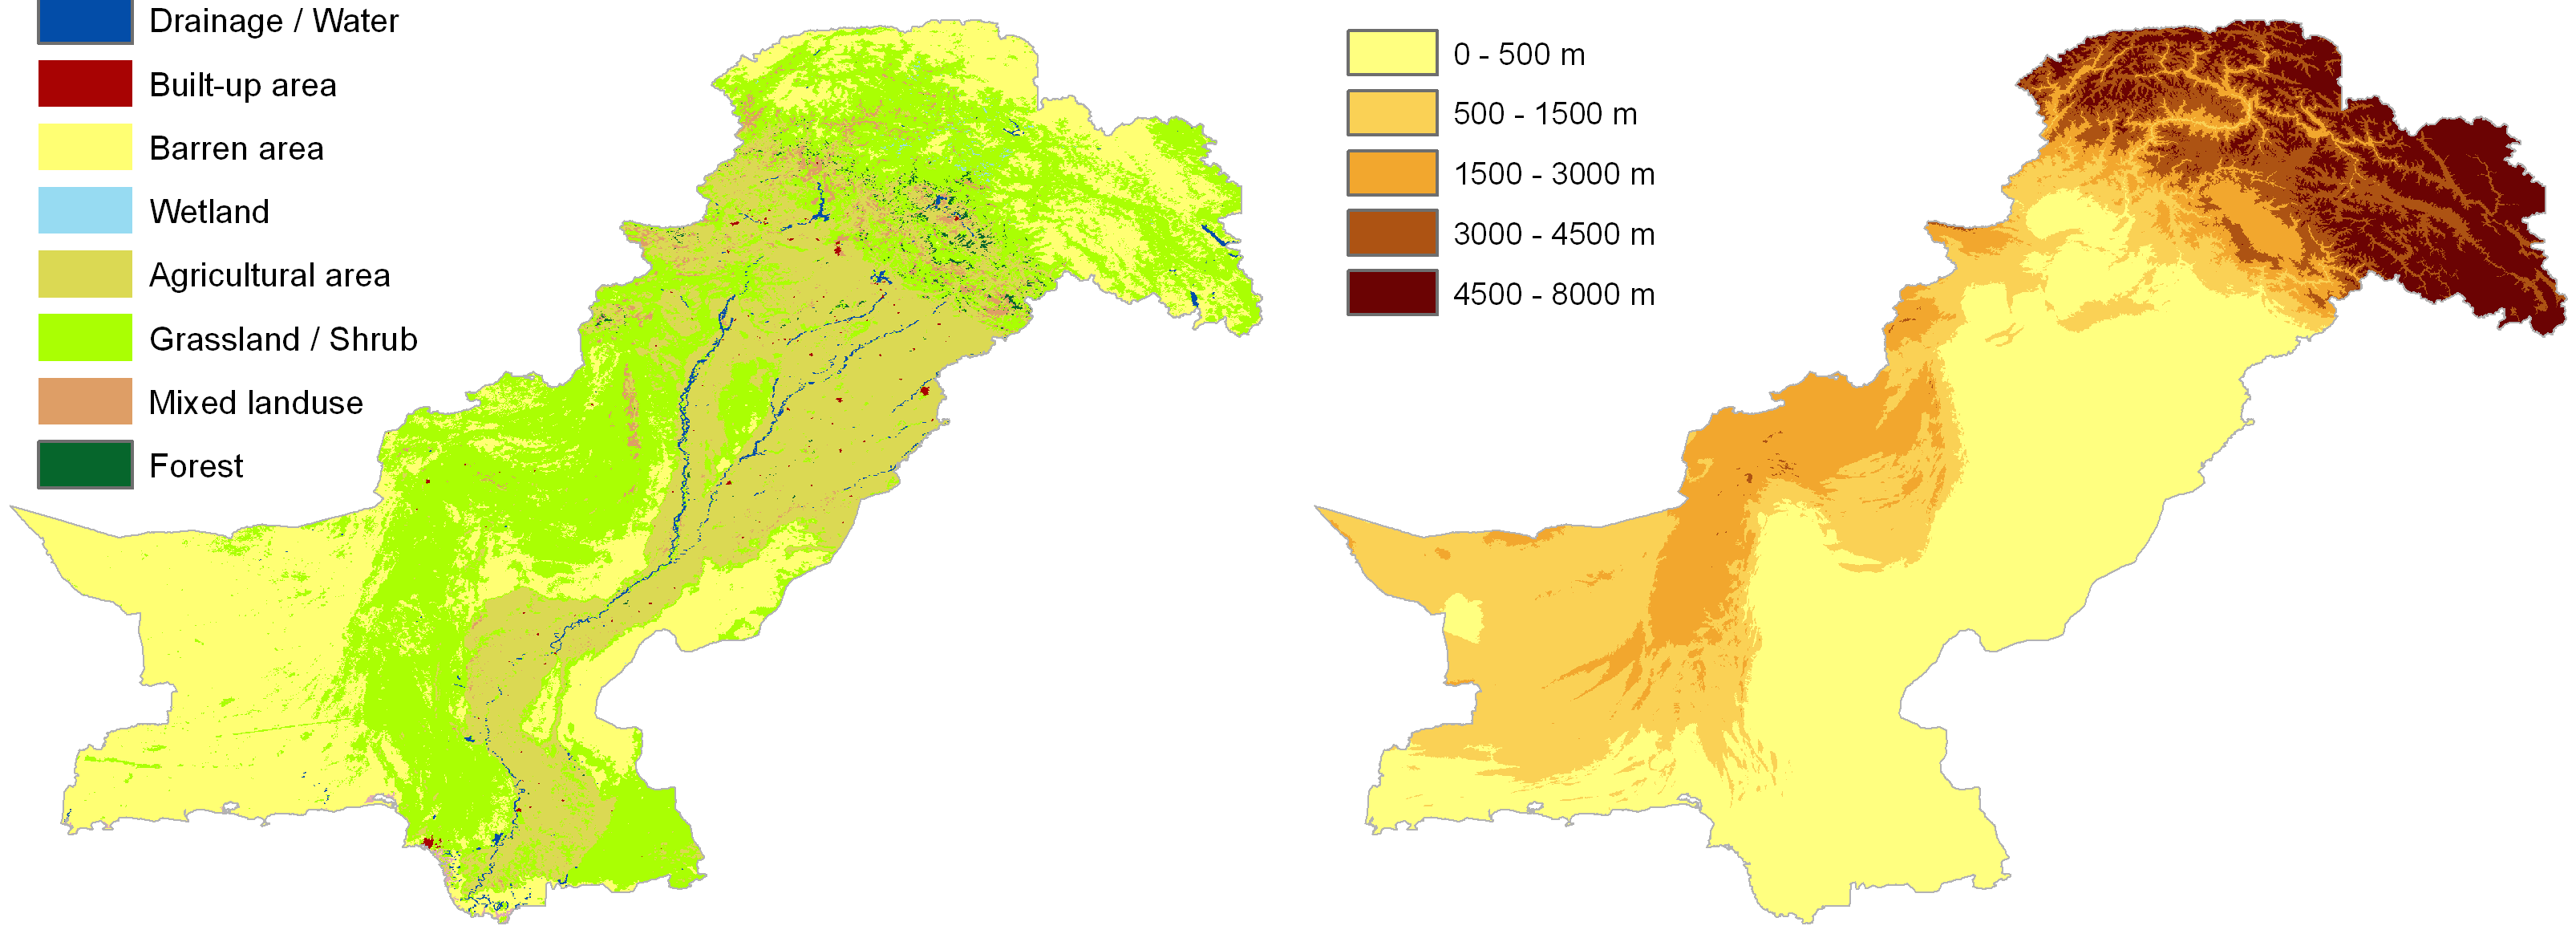
\includegraphics[width=1.05\textwidth]{images/Spatial_predictors.png} \\
  \alert{Land cover \footnotesize{(ISCGM, 2014)}} BL, AL, ML \hspace{4pt} \alert{Elevation \footnotesize{(Rodriguez et al., 2005. Science)}} \\
  \pause
  \alert{Global soil properties \footnotesize{(Batjes, 2000. ISRIC)}} SOC, SCC, WC, pH
\end{frame}

%%%%%%%%%%%%%%%%%%%%%%%%%%% Slide 26 %%%%%%%%%%%%%%%%%%%%%%%%%

%\begin{frame}[fragile]
 % \frametitle{We calibrated local GWR models \protect\\ and used them for spatial prediction}
  %\begin{equation*}
   % C_{T,z} = \delta_{z,0} + \sum_{n=1}^{m=8}\delta_{z,n}S_{z,n} + e_z
    %\end{equation*}
  %\begin{itemize}
   %     \item \alert{Gaussian kernel} based on the spatial continuity
    %    \pause
     %   \item \alert{Fixed kernel bandwidths} based on AIC
      %  \pause
       % \item \alert{Best-fit models} forward entering of spatial predictors and based on AIC \\
        %\centering e.g. Cr\_SW\textasciitilde WC + ALU \\
        %\pause
        %\raggedright
        %\item \alert{R package GWmodel} (Gollini et al. 2013)
      %\end{itemize}
%\end{frame}

%%%%%%%%%%%%%%%%%%%%%%%%%%% Slide 27 %%%%%%%%%%%%%%%%%%%%%%%%%

%\begin{frame}{We evaluated prediction accuracy and uncertainty by \protect\\ leave-one-out cross-validation}
 %     \begin{itemize}
  %      \item  perfect agreement 1, no agreement 0
   %     \pause
    %    \item  lower value indicates higher accuracy
     %   \pause
      %  \item unity indicates high certainty
      %\end{itemize}
%\end{frame}

%%%%%%%%%%%%%%%%%%%%%%%%%%% Slide 28 %%%%%%%%%%%%%%%%%%%%%%%%%

\begin{frame}[fragile]
  \frametitle{We estimated area and population at risk \protect\\ by comparing to ``WHO'' guideline thresholds}
  \centering
  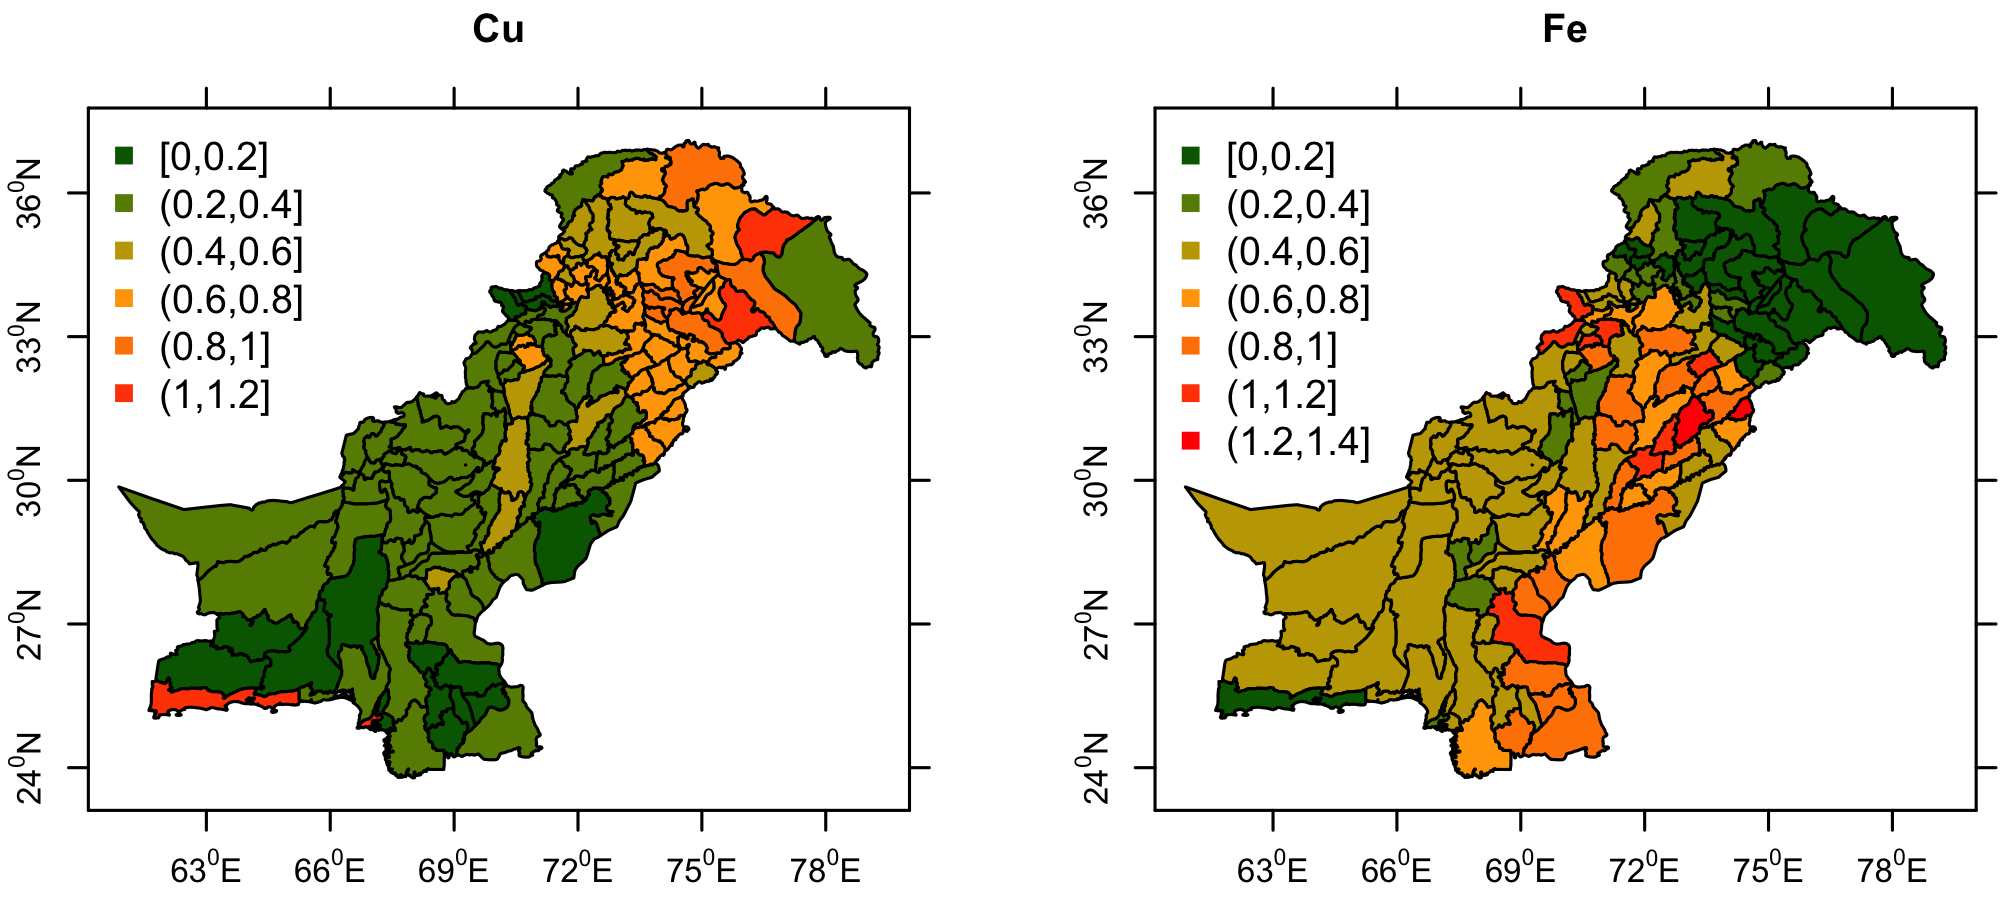
\includegraphics[width=0.9\textwidth]{images/Prediction_example.png}\\
  Model validation: \small \alert{Index of agreement ($d$)}, \alert{Root mean squared deviation error ($RMSDE$)} and \alert{Standard deviation of prediction z-scores ($SDZ$)}\\
  \pause \vspace{-0.3cm} \normalsize
  \begin{equation*}
    RQ_{T,z} = \frac{\hat{C}_{z,0}}{C_{WHO-T}}
    \end{equation*}\\
  \alert{RQ>1} at risk \alert{RQ $\leq$ 1} negligible risk \footnotesize{(WHO, 2011)}
\end{frame}

%%%%%%%%%%%%%%%%%%%%%%%%%%% Slide 29 %%%%%%%%%%%%%%%%%%%%%%%%%

\begin{frame}
  \frametitle{More than 53 \% of total area and 74 million people \protect\\ are at risk from arsenic, chromium, iron, nickel and lead}
  \centering 
  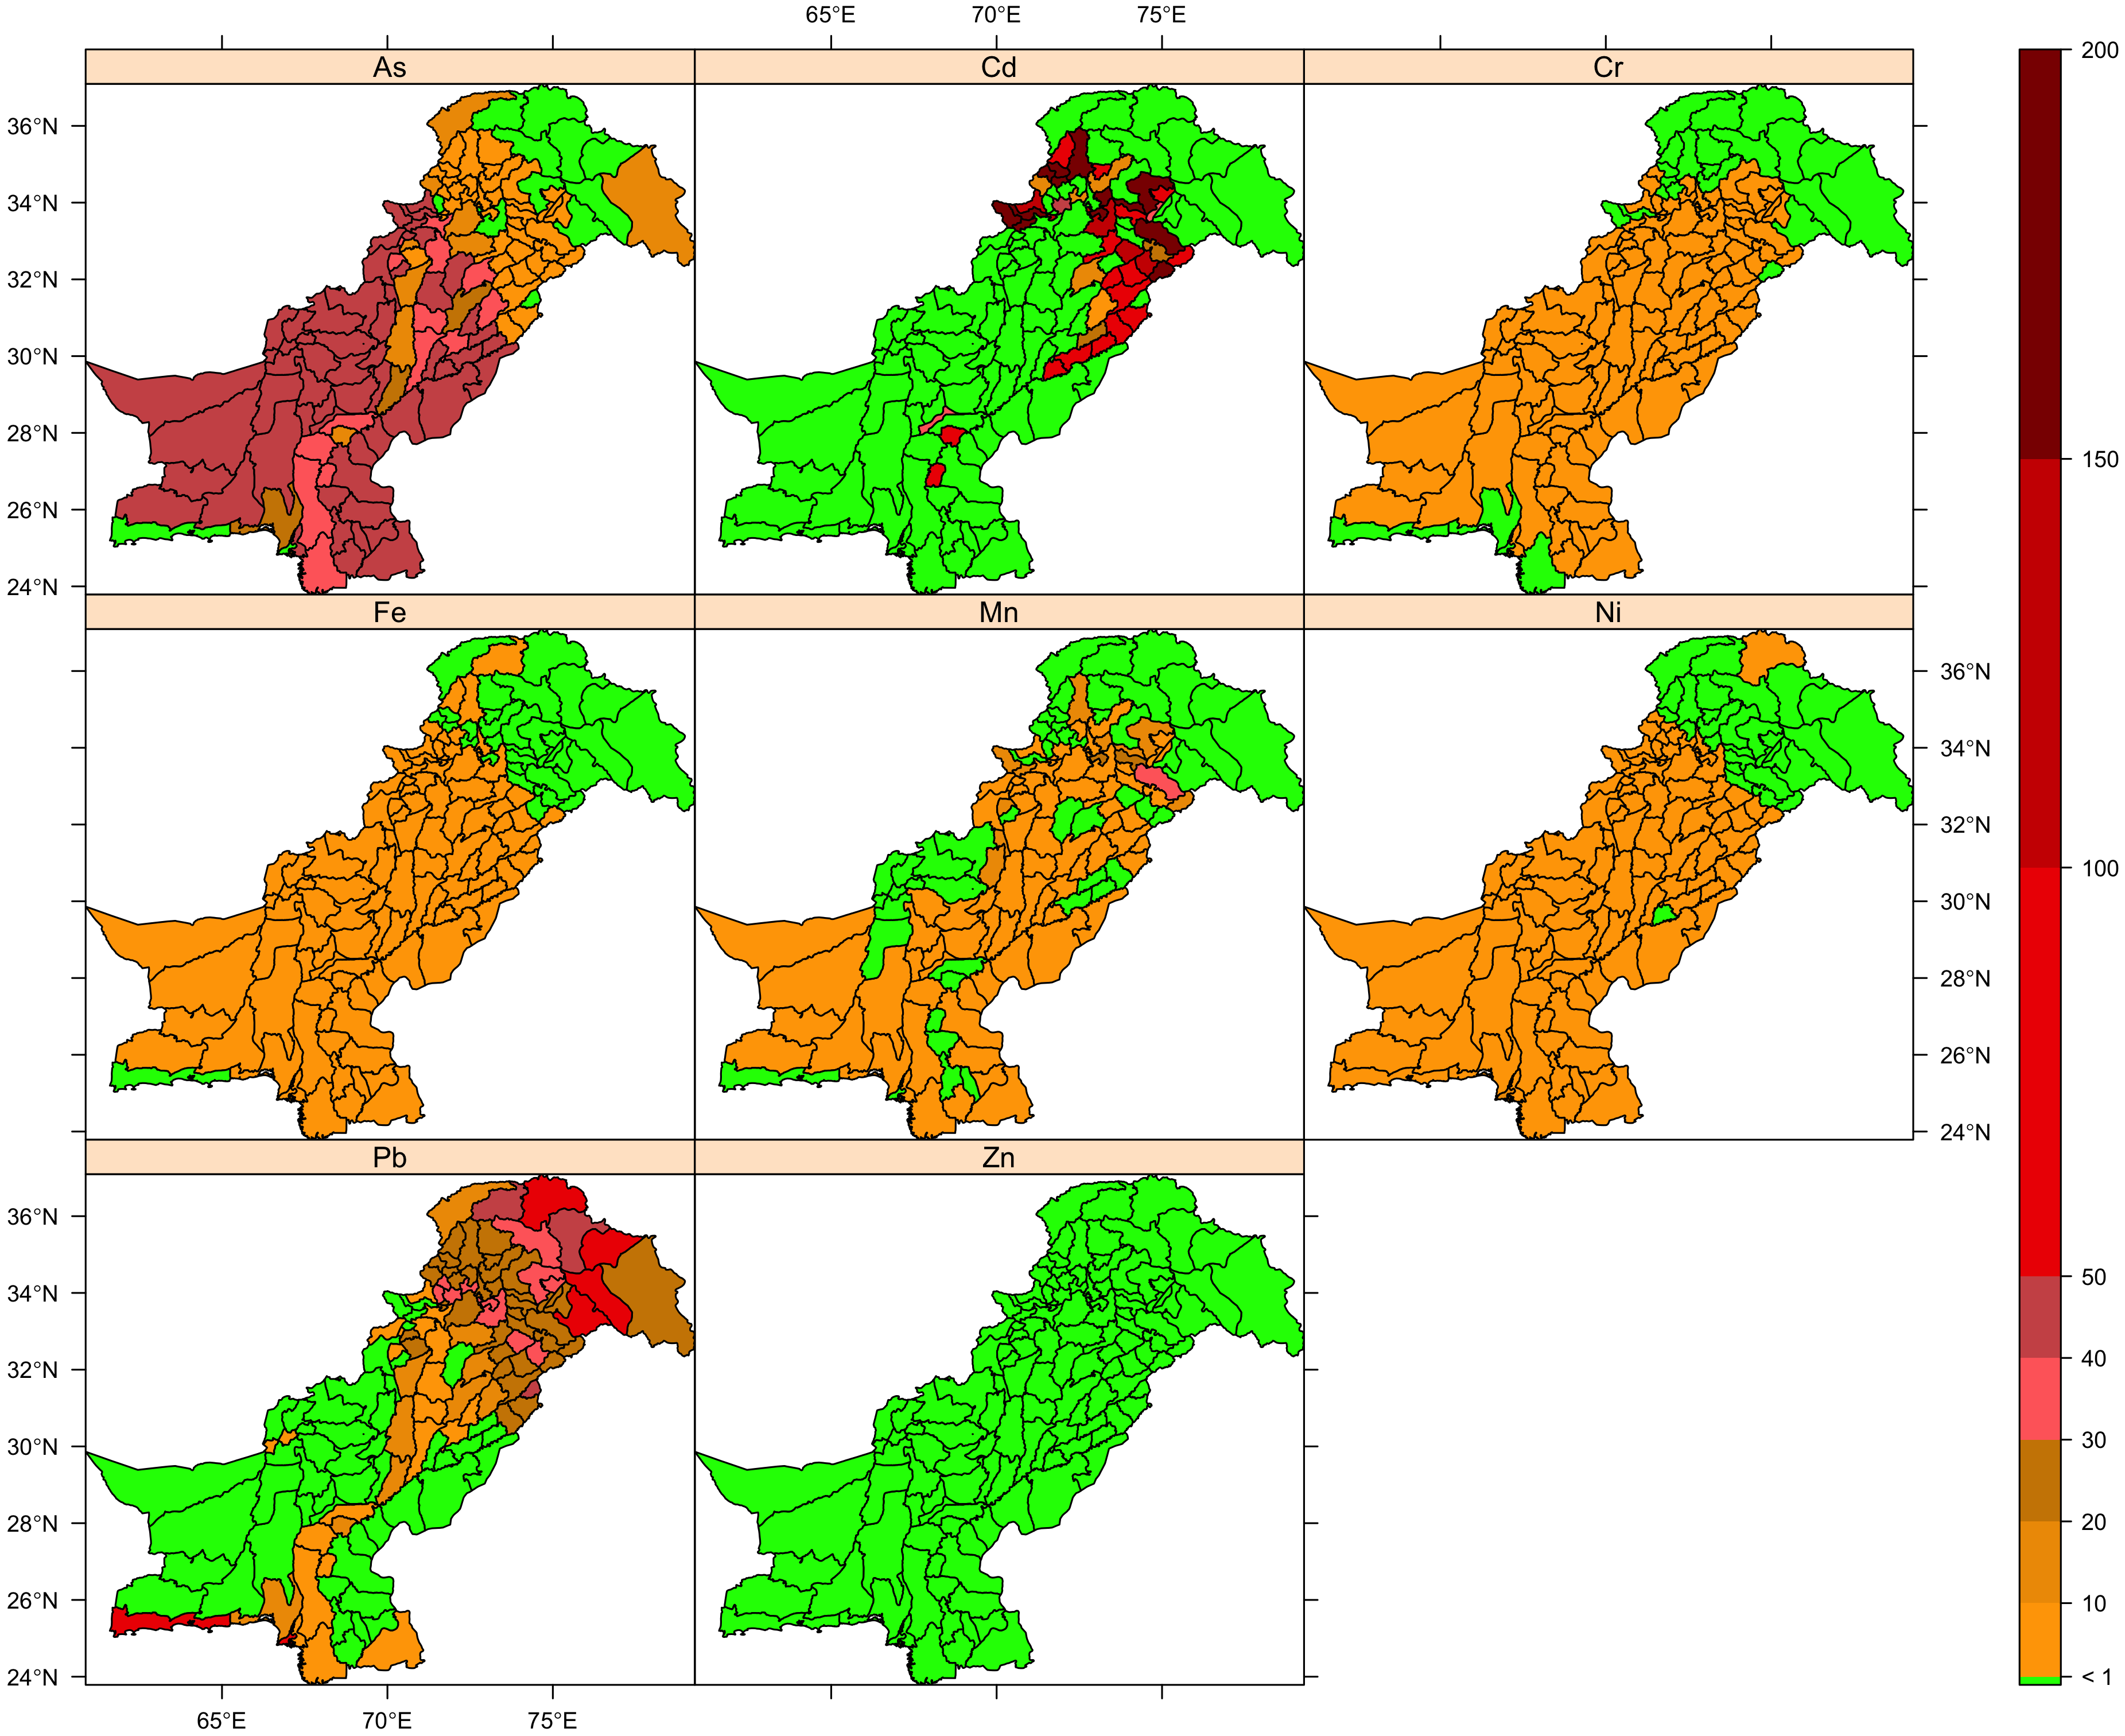
\includegraphics[width=0.84\textwidth]{images/Ground_water_risk.png}
\end{frame}

%%%%%%%%%%%%%%%%%%%%%%%%%%% Slide 30 %%%%%%%%%%%%%%%%%%%%%%%%%

\begin{frame}
  \frametitle{More than 53 \% of total area and 74 million people \protect\\ are at risk from arsenic, chromium, iron, nickel and lead}
  \centering
  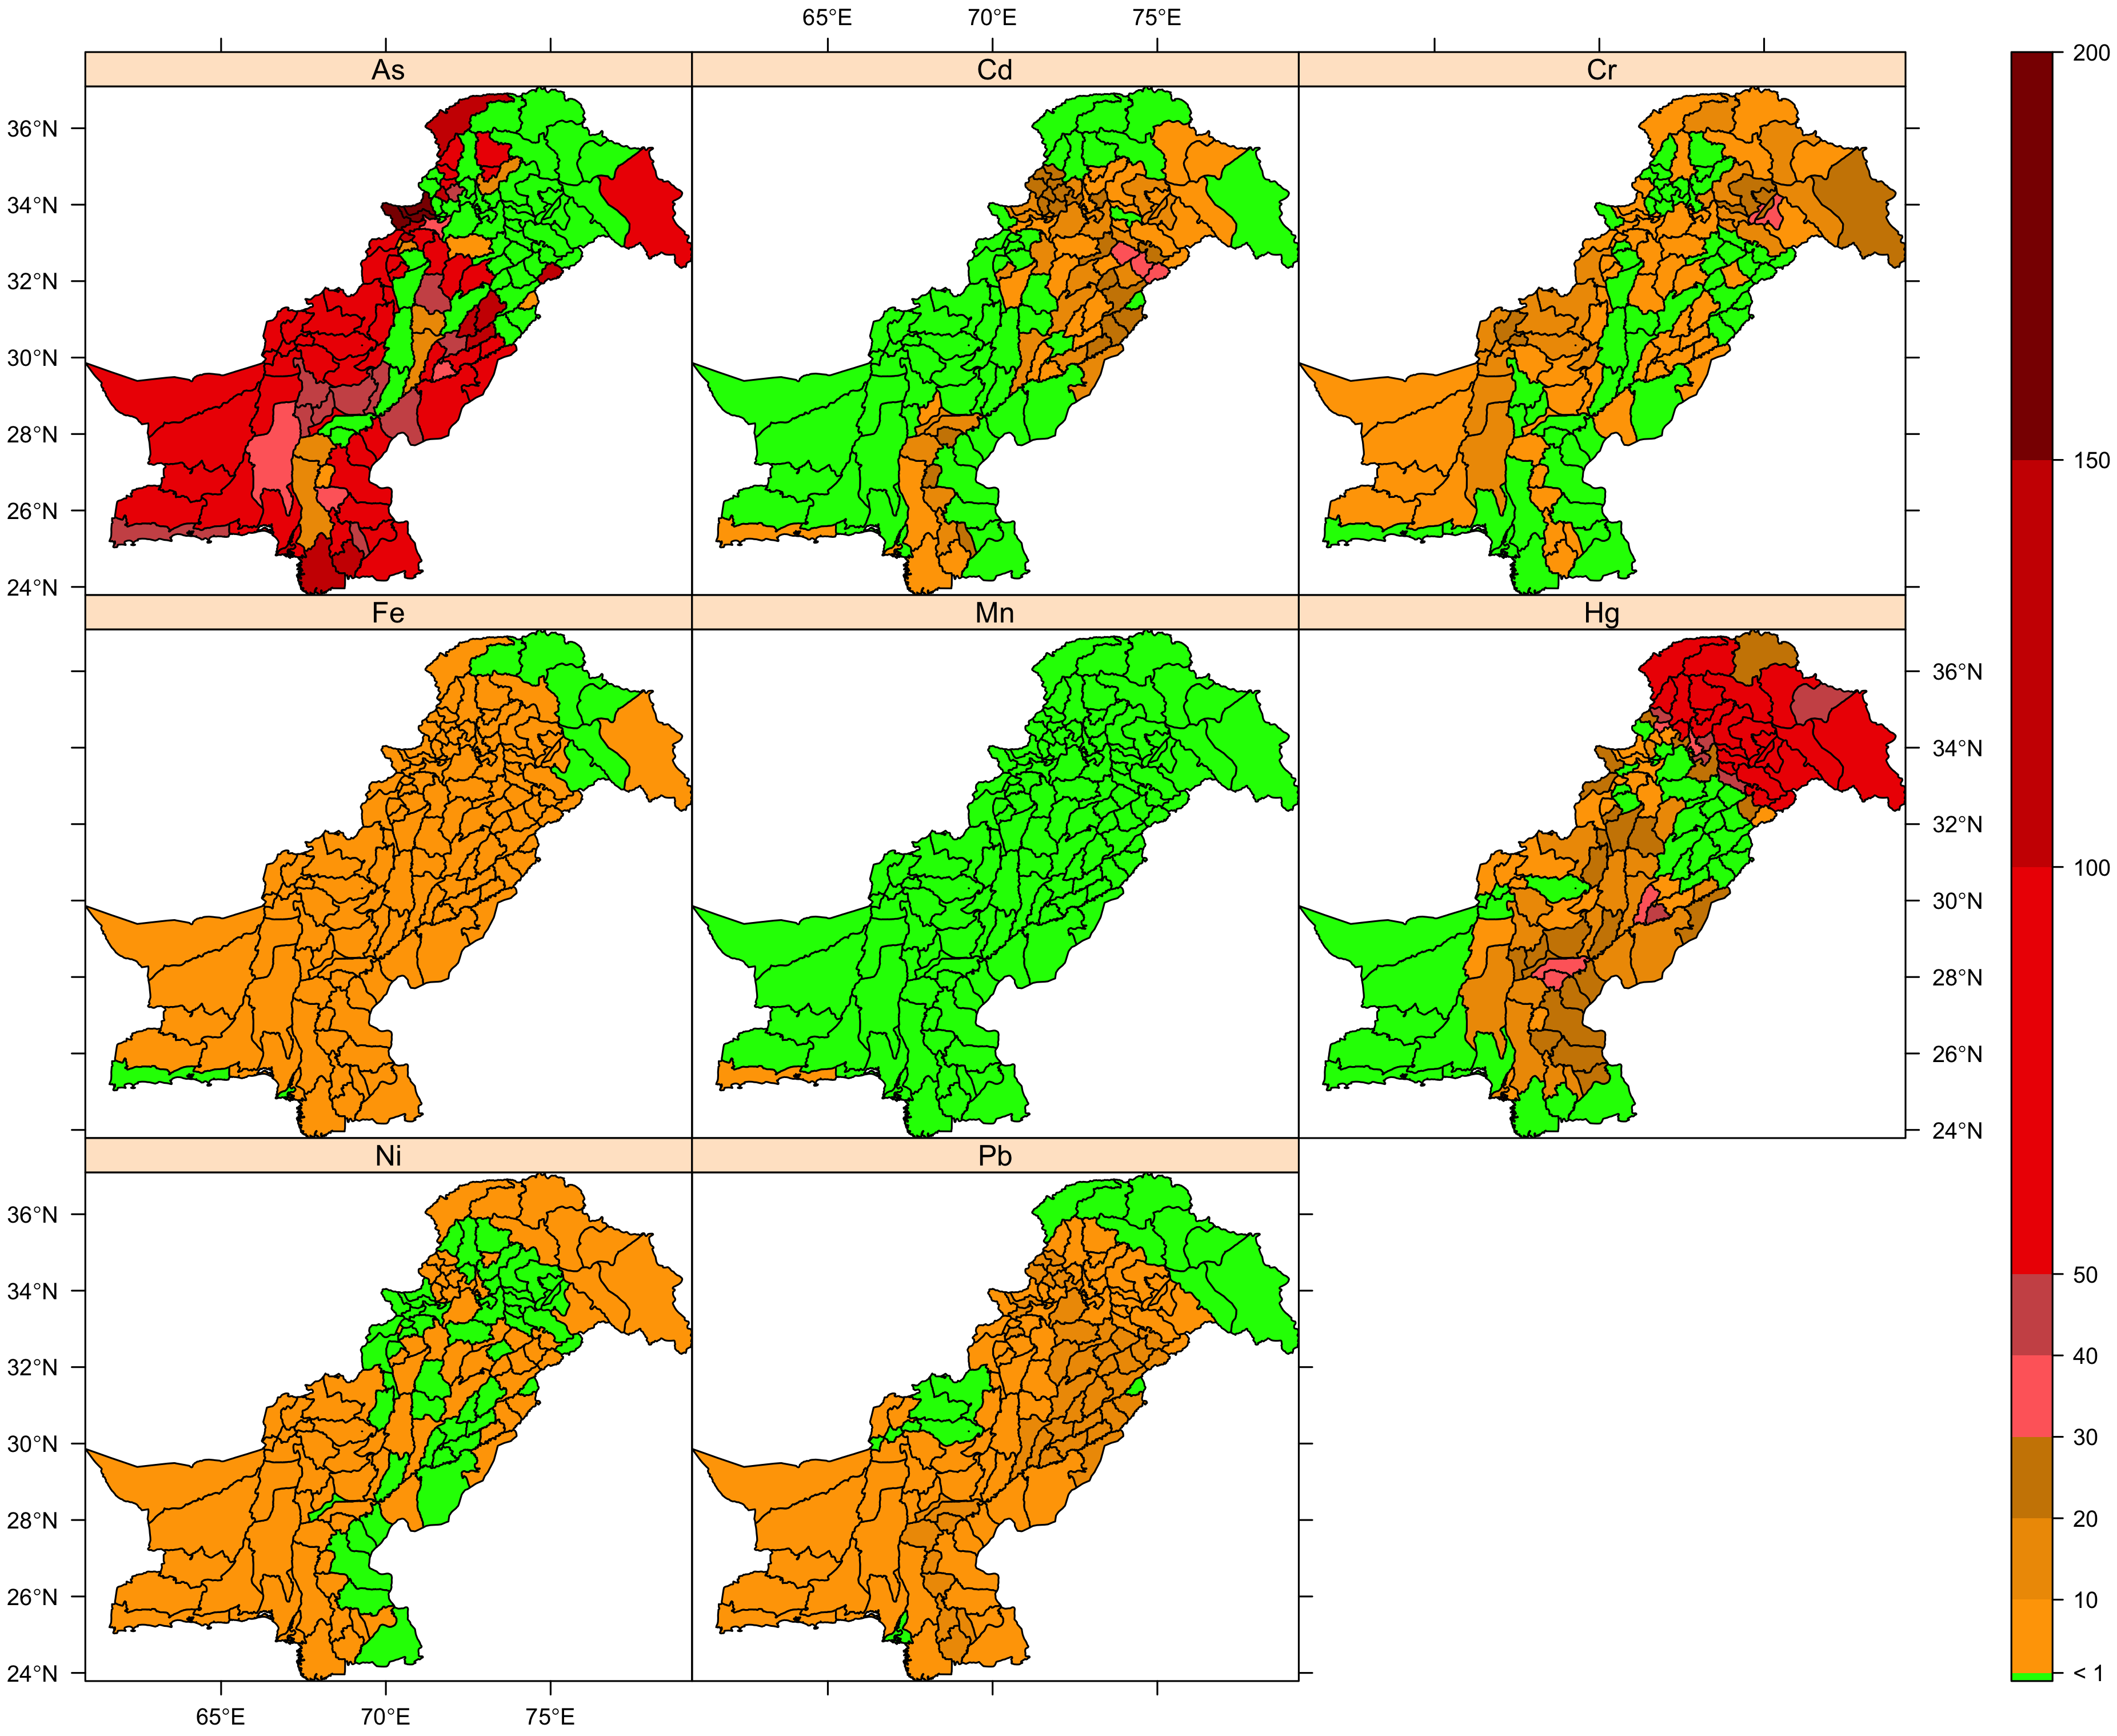
\includegraphics[width=0.84\textwidth]{images/Surface_water_risk.png}
\end{frame}

%%%%%%%%%%%%%%%%%%%%%%%%%%% Slide 31 %%%%%%%%%%%%%%%%%%%%%%%%%

\begin{frame}{Our GWR model predictions exhibited a high accuracy \protect\\ and a low uncertainty}
  %\begin{columns}[onlytextwidth]
    %\column{0.5\textwidth}
      %Items
      \begin{itemize}
        \item \alert{$d$ \geq 0.8} except for iron in ground water and zinc in surface water
        \pause
        \item \alert{$RMSDE$ \leq 0.45} 0.97 for iron in ground water and 0.8 for zinc in surface water
        \pause
        \item \alert{$SDZ$ \geq 0.7} except for cadmium and zinc in ground water, and cadmium and manganese in surface water
        \pause
        \item \alert{Calibrated spatial predictors are in agreement with the causes of trace metal contamination} e.g. As\_SW\textasciitilde SOC + pH \\ \footnotesize (Husain et al. 2012. Int. J. Ecol. Env. Geol.)
      \end{itemize}
\end{frame}

%%%%%%%%%%%%%%%%%%%%%%%%%%% Slide 32 %%%%%%%%%%%%%%%%%%%%%%%%%

\begin{frame}{The predictions inform water resources management \protect\\ on potential hot spots}
      \begin{itemize}
        \item \alert{Predictions may not reflect true trace metal concentration variation} 453 km $\leq$ kernel bandwidth $\leq$ 1335 km \\ \footnotesize (Bhowmik and Costa, 2014. Met. App.)\normalsize
        \pause
        \item \alert{Predictions complement field monitoring} although require field validation
        \pause
        \item \alert{Predictions with low accuracy and high uncertainty need to be treated with caution} e.g. zinc
        \pause
        \item \alert{Perhaps over-prediction for areas with access to water purification} more relevant for rural areas \footnotesize (Khan et al., 2012. Env. Pol.) \normalsize
        \pause
        \item \alert{May also indicate indirect effects} e.g. via consumption of vegetables irrigated with contaminated water \footnotesize (Amin et al., 2012. ASSET)\normalsize
      \end{itemize}
\end{frame}

%%%%%%%%%%%%%%%%%%%%%%%%%%%%%%%%%%%%%%%%%%%%%%%%%%%%%%%%%

\begin{frame}{Freshwater degradation is alarming \protect\\ Science can act Pro}
\begin{center}
\includemedia[width=1.2\textheight, height=.7\textheight,activate=pagevisible, deactivate=pageclose, addresource=video/FD.mp4, flashvars={src=video/FD.mp4 &autoPlay=true &loop=true &controlBarAutoHideTimeout=0}]{}{StrobeMediaPlayback.swf}
\end{center}
\end{frame}

%%%%%%%%%%%%%%%%%%%%%%%%%%%%%%%%%%%%%%%%%%%%%%%%%%%%%%%%%

\begin{frame}{Future research challenges}
\begin{itemize}
\item Trait convergence, Aquatic - terrestrial interaction \\ and Trait potential to distinguish between stressors\\
\vspace{0.5cm}
\item Filling data gaps: Crowd-sourced data
\end{itemize}
\end{frame}

%%%%%%%%%%%%%%%%%%%%%%%%%%%%%%%%%%%%%%%%%%%%%%%%%%%%%%%%%

\plain{}{\LARGE Thank You\\
\vspace{15pt}
\raggedright
\begin{columns}
\column{5cm}
\normalsize Jun. Prof. Dr. Ralf B. Schäfer\\
Dr. Markus Metz\\
Dr. S. A. M. A. S. Eqani\\
\\ \vspace{0.3cm}
The open-source and\\
\LARGE R \normalsize community\\ \vspace{0.5cm}

\includegraphics[width=0.8\textwidth]{images/logo.png}
\column{5cm}
\includegraphics[width=1.1\textwidth]{images/AGLE.png}
\end{columns}}

%%%%%%%%%%%%%%%%%%%%%%%%%%%%%%%%%%%%%%%%%%%%%%%%%%%%%%%%%

\end{document}

%%%%%%%%%%%%%%%%%%%%%%%%%%%%%%%%%%%%%%%%%%%%%%%%%%%%%%%%%
%%%%%%%%%%%%%%%%%%%%%%%%%%% End %%%%%%%%%%%%%%%%%%%%%%%%%
%%%%%%%%%%%%%%%%%%%%%%%%%%%%%%%%%%%%%%%%%%%%%%%%%%%%%%%%%
